% ============================================================
% Informe de Proyecto Final
% Cloud Computing (MCD8007) - UTEC Posgrado
% ============================================================
\documentclass[12pt,letterpaper]{article}

\usepackage[utf8]{inputenc}
\usepackage[spanish]{babel}
\addto\captionsspanish{\renewcommand{\tablename}{Tabla}}
\addto\captionsspanish{\renewcommand{\listtablename}{Índice de tablas}}
\usepackage{graphicx}
\usepackage{fancyhdr}
\usepackage{geometry}
\usepackage[hidelinks]{hyperref}
\usepackage{booktabs}
\usepackage{array}
\usepackage{listings}
\usepackage{xcolor}
\usepackage{float}
\usepackage{setspace}
\usepackage{enumitem}
\usepackage{caption}
\usepackage{amsmath}
\usepackage{needspace}
\usepackage{microtype}
\usepackage{tikz}
\usepackage{tocloft}
\setlength{\cftbeforesecskip}{3pt}
\setlength{\cftbeforesubsecskip}{1pt}
\renewcommand{\cftsecafterpnum}{\hfill}
\usetikzlibrary{arrows.meta, positioning, fit, backgrounds, calc}

\geometry{left=2.3cm, right=2.3cm, top=2.5cm, bottom=2.5cm}
\setlength{\parskip}{6pt}
\setlength{\parindent}{0pt}
\onehalfspacing

\setlength{\headheight}{14.5pt}
\pagestyle{fancy}
\fancyhf{}
\fancyhead[L]{SiniestroExpress / Proyecto Final}
\fancyhead[R]{\thepage}
\renewcommand{\headrulewidth}{0.5pt}

\definecolor{codebg}{rgb}{0.95,0.95,0.95}
\definecolor{codeframe}{rgb}{0.8,0.8,0.8}
\definecolor{codecomment}{rgb}{0.35,0.55,0.35}
\definecolor{codekw}{rgb}{0.0,0.0,0.65}
\lstdefinestyle{mystyle}{
    backgroundcolor=\color{codebg},
    frame=single,
    rulecolor=\color{codeframe},
    basicstyle=\ttfamily\footnotesize,
    breakatwhitespace=false,
    breaklines=true,
    keepspaces=true,
    showspaces=false,
    showstringspaces=false,
    showtabs=false,
    tabsize=2,
    inputencoding=utf8,
    extendedchars=true,
    commentstyle=\color{codecomment}\itshape,
    keywordstyle=\color{codekw}\bfseries,
    literate={á}{{\'a}}1 {é}{{\'e}}1 {í}{{\'i}}1 {ó}{{\'o}}1 {ú}{{\'u}}1 {ñ}{{\~n}}1 {Á}{{\'A}}1 {É}{{\'E}}1 {Í}{{\'I}}1 {Ó}{{\'O}}1 {Ú}{{\'U}}1 {ü}{{\"u}}1 {º}{{\textordmasculine}}1 {¿}{{?`}}1 {¡}{{!`}}1
}
\lstset{style=mystyle}

\newcommand{\code}[1]{\texttt{\detokenize{#1}}}

\hypersetup{
  pdftitle={SiniestroExpress: triaje agéntico de siniestros vehiculares},
  pdfauthor={Sebastian Rodrigo Garcia Villacorta, Dante Guillermo Barreto Daza,
  Clinton Michael Chulluncuy Reynoso, Ronald Ramiro Hilario Orihuela}
}

\begin{document}

% ============================================================
% CARÁTULA
% ============================================================
\begin{titlepage}
\centering

\vspace*{0.3cm}


\includegraphics[width=4.5cm]{utec-logo.png}\\[0.5cm]

{\Large\bfseries UNIVERSIDAD DE INGENIER\'IA Y TECNOLOG\'IA}\\[0.1cm]
{\large\bfseries ESCUELA DE POSGRADO}\\[1cm]

\rule{\textwidth}{1pt}\\[0.4cm]
{\normalsize\bfseries SiniestroExpress: triaje agéntico de siniestros vehiculares}\\[0.1cm]
{\normalsize\bfseries Diseño e implementación de un workflow agéntico serverless en AWS}\\[0.4cm]
\rule{\textwidth}{1pt}\\[1.2cm]

\vfill

{\normalsize\bfseries INTEGRANTES}\\[0.3cm]
\begin{tabular}{l}
Sebastian Rodrigo Garcia Villacorta\\
Dante Guillermo Barreto Daza\\
Clinton Michael Chulluncuy Reynoso\\
Ronald Ramiro Hilario Orihuela
\end{tabular}\\[0.6cm]

{\normalsize\bfseries DOCENTE}\\[0.2cm]
{\normalsize Oscar Rodolfo Mejía Fernández}\\[0.6cm]

{\normalsize\bfseries CURSO}\\[0.2cm]
{\normalsize Cloud Computing (MCD8007)}\\[1cm]

\vfill

{\normalsize Lima --- Per\'u, 2026}

\end{titlepage}

\section*{Resumen ejecutivo}
\addcontentsline{toc}{section}{Resumen ejecutivo}

Cobrar un seguro de auto debería tomar minutos, pero en el mercado peruano toma días.
El asegurado llama, cuenta lo que pasó tres veces, espera a que un perito lo visite y
recibe el dinero varias semanas después. SiniestroExpress convierte ese trámite en una
conversación: el asegurado entra con su número de póliza, cuenta qué le pasó y, en la
misma pantalla, recibe el monto que le corresponde, la ruta de atención y un código para
seguir el caso.

El sistema se compone de tres servicios desplegados sobre AWS: un agente conversacional
que utiliza la API de Groq con memoria en DynamoDB, un servicio de negocio que administra
pólizas y expedientes, y un servicio de modelos que estima el costo de reparación y la
probabilidad de abandono. Los tres corren en Lambda con API Gateway y DynamoDB, sin un
solo servidor encendido. El paquete completo de modelos pesa 2,4 MB porque los bosques se
exportaron a JSON y se evalúan con la biblioteca estándar de Python: la alternativa con
scikit-learn superaba el límite de 50 MB de Lambda.

Los modelos se entrenaron con 1,000 siniestros sintéticos, cuyos montos se recalcularon
con precios de taller de Lima. El modelo de costo alcanza un error absoluto medio de
S/. 394 y un coeficiente de determinación de 0,95. El motor de decisión se calibró con los
percentiles de esa misma distribución, de modo que los umbrales de pago exprés y de
peritaje no son cifras elegidas a mano.

El proyecto se implementó, se desplegó y se probó de extremo a extremo. Las 50 pruebas
automatizadas pasan y las 19 peticiones de la colección de Postman cubren el flujo
completo, incluidos los casos que deben fallar.

\clearpage
{\small
\tableofcontents
}
\thispagestyle{fancy}

% ============================================================
% PARTE A
% ============================================================
\clearpage
\section{Parte A: análisis}

\subsection{La empresa y la problemática}

\textbf{Andes Seguros} es una aseguradora ficticia del ramo vehicular con 32,000 pólizas
vigentes y cerca de 1,900 siniestros al mes. Su operación de siniestros está organizada
en cuatro pasos: recepción telefónica, registro, inspección y liquidación. Cada paso
tiene su propio correo y su propio archivo.

El problema no es la falta de información, sino la fricción entre esas islas. Un caso
típico de daño parcial sigue este recorrido:

\begin{enumerate}[itemsep=2pt]
  \item El asegurado llama a la central y dicta su versión a un operador que llena un
        formulario de 34 campos.
  \item El analista revisa el caso al día siguiente, encuentra un dato incoherente y
        vuelve a llamar para confirmarlo.
  \item Se asigna un perito, que agenda una visita según la zona y la agenda del taller.
  \item El perito emite un informe que alguien transcribe a otro sistema.
  \item Liquidación calcula el monto y lo envía a pagos.
\end{enumerate}

El resultado medido en el piloto de tres meses: \textbf{once días promedio} entre el
aviso y el depósito, con un 18 \% de casos que supera los 20 días. La Ley 29946 de
contrato de seguro fija un plazo de 30 días para la indemnización, de modo que el proceso
opera cerca del límite legal. Además, la encuesta de salida del piloto muestra que el
22 \% de los asegurados con un siniestro no renueva su póliza al año siguiente, frente al
9 \% de quienes no lo tienen.

El costo interno también esconde una ineficiencia: cada caso consume unos
\textbf{1.2 horas de trabajo administrativo} por caso. De ese tiempo, más de la mitad se va
en tareas que no agregan valor: volver a preguntar, transcribir y perseguir documentos.

\subsection{El workflow agéntico}

El workflow se llama \textbf{SiniestroExpress} y corresponde al \textbf{Nivel 3} de
sofisticación: API de modelo de lenguaje con memoria conversacional, invocación de APIs
de modelos de machine learning entrenados fuera de línea, y persistencia en una base de
datos propia.

Un workflow agéntico es aquel en el que un modelo de lenguaje no solo redacta, sino que
decide cuándo ya tiene la información suficiente, qué pregunta falta y qué acción
disparar. En SiniestroExpress el agente conversa y el sistema decide: el modelo nunca
calcula montos ni aprueba pagos, porque esa parte se resuelve con reglas que se pueden
auditar.

\subsection{Benchmark de alternativas}

Antes de elegir AWS se compararon tres alternativas de automatización no vinculadas a la
nube de Amazon. La comparación no busca un ganador absoluto, sino entender qué tipo de
herramienta resuelve el problema.

\begin{table}[H]
\centering
\caption{Comparación de alternativas de automatización}
\label{tab:benchmark}
\small
\begin{tabular}{p{2.5cm}p{3.4cm}p{3.6cm}p{4.2cm}}
\toprule
\textbf{Alternativa} & \textbf{Enfoque} & \textbf{Lo que resuelve bien} & \textbf{Dónde no alcanza} \\
\midrule
n8n (autoalojado) &
Flujos por nodos con disparadores, ejecutado en un contenedor propio &
Integraciones rápidas sin escribir código; control total del despliegue &
Requiere un servidor siempre encendido, parcheo y respaldo propios; el costo no escala a cero \\
\addlinespace
Make &
Automatización en la nube por operaciones &
Conectores listos y editor visual; buena experiencia para procesos administrativos &
El cobro por operación penaliza la conversación de varios turnos; el razonamiento del agente queda fuera de su alcance \\
\addlinespace
Zapier Central &
Agentes sobre aplicaciones de terceros &
Rapidez para conectar correo, hojas de cálculo y mensajería &
Poca libertad sobre el modelo, los datos y la lógica de decisión; los datos salen del control de la aseguradora \\
\addlinespace
AWS (elegida) &
Servicios desacoplados por evento: Lambda, API Gateway, DynamoDB y S3 &
Control del modelo y de las reglas, pago por uso y escalado automático sin servidores &
Exige desarrollo propio y una curva de aprendizaje sobre IAM y empaquetado \\
\bottomrule
\end{tabular}
\end{table}

La lectura es directa: las herramientas de automatización resuelven la \emph{conexión}
entre sistemas, pero el problema de Andes Seguros es la \emph{decisión}. Nadie gana
conectando el formulario con el correo si el caso sigue esperando a un perito que no hacía
falta. Por eso se eligió una arquitectura propia sobre AWS, donde el modelo, las reglas y
los datos quedan bajo control de la aseguradora.

\subsection{Tipos de clientes y usuarios}

\begin{table}[H]
\centering
\caption{Usuarios del sistema y lo que necesitan}
\label{tab:usuarios}
\small
\begin{tabular}{p{2.6cm}p{4.2cm}p{6.6cm}}
\toprule
\textbf{Usuario} & \textbf{Contexto} & \textbf{Necesidad principal} \\
\midrule
Asegurado & Acaba de tener un siniestro; está en la calle, desde el celular &
Saber cuánto le van a pagar y cuándo, sin trámites ni llamadas \\
\addlinespace
Analista & Revisa casos remotos en jornada de ocho horas &
Recibir el caso ya armado, con monto sugerido y evidencia, y poder aprobarlo o rechazarlo \\
\addlinespace
Coordinador & Supervisa la cola y los plazos &
Ver cuántos casos hay por estado, cuáles están por vencer y cuánto se está pagando \\
\addlinespace
Administrador & Mantiene pólizas y usuarios &
Cargar y actualizar pólizas, revisar la operación y exportar datos para auditoría \\
\bottomrule
\end{tabular}
\end{table}

\subsection{Funcionalidades e historias de usuario}

Se definieron ocho historias de usuario que cubren el recorrido completo. Cada una tiene
su criterio de aceptación en formato Gherkin.

\begin{table}[H]
\centering
\caption{Historias de usuario del MVP}
\label{tab:hu}
\small
\begin{tabular}{p{1.3cm}p{4.6cm}p{7.6cm}}
\toprule
\textbf{ID} & \textbf{Historia} & \textbf{Criterio de aceptación} \\
\midrule
HU-01 & Como asegurado quiero identificarme con mi póliza para no llenar un formulario &
Con un número de póliza válido el sistema muestra marca, modelo y año del vehículo \\
\addlinespace
HU-02 & Como asegurado quiero contar qué pasó en mis palabras &
El agente extrae tipo de siniestro, severidad y piezas de un relato libre \\
\addlinespace
HU-03 & Como asegurado quiero una pregunta por turno y no repetir lo ya dicho &
El agente no vuelve a preguntar un dato ya extraído \\
\addlinespace
HU-04 & Como asegurado quiero saber cuánto voy a cobrar y en cuánto tiempo &
Al cerrar la conversación el sistema muestra monto a pagar, ruta y plazo \\
\addlinespace
HU-05 & Como asegurado quiero seguir mi caso sin llamar &
Con el código de seguimiento el sistema muestra el estado y la conversación \\
\addlinespace
HU-06 & Como asegurado quiero adjuntar fotos del daño &
Puedo elegir, revisar y quitar fotos antes de enviarlas \\
\addlinespace
HU-07 & Como analista quiero la cola por estado y el detalle de cada caso &
El panel lista los expedientes y filtra por estado \\
\addlinespace
HU-08 & Como analista quiero aprobar o rechazar con un clic &
El backend impide aprobar un caso ya rechazado y lo informa \\
\bottomrule
\end{tabular}
\end{table}

El escenario principal, escrito en Gherkin:

\begin{lstlisting}[language=bash, caption={Escenario de pago exprés}, label={lst:gherkin1}]
Característica: Triaje de un siniestro con daño leve
  Como asegurado
  Quiero reportar un choque menor
  Para cobrar sin esperar una inspeccion

  Escenario: Choque leve con dos piezas y sin grua
    Dado que ingreso mi póliza "AUTO-2026-8801"
    Y cuento que "me chocaron por atras, fue leve, dos piezas, no necesite grua"
    Cuando el agente extrae los datos del relato
    Entonces el sistema registra 2 piezas afectadas
    Y la severidad queda en "Leve"
    Y la ruta asignada es "Pago exprés"
    Y el plazo informado es de 24 horas
    Y recibo un código de seguimiento con formato "SE-XXXXXX"
\end{lstlisting}

\begin{lstlisting}[language=bash, caption={Escenario de documentación pendiente}, label={lst:gherkin2}]
  Escenario: Robo de piezas sin parte policial
    Dado que cuento que "me robaron las llantas"
    Cuando el agente detecta que falta el parte policial
    Entonces el estado queda en "Documentación pendiente"
    Y el sistema me pide ese documento antes de liquidar
    Y no me muestra un monto definitivo
\end{lstlisting}

\begin{lstlisting}[language=bash, caption={Escenario de transición no permitida}, label={lst:gherkin3}]
  Escenario: Un caso rechazado no puede aprobarse
    Dado un expediente en estado "Rechazado"
    Cuando el analista intenta aprobarlo
    Entonces el backend responde 409
    Y explica el estado actual y las acciones permitidas
\end{lstlisting}

\subsection{Propuesta de valor}

\begin{table}[H]
\centering
\caption{Propuesta de valor frente al proceso actual}
\label{tab:valor}
\small
\begin{tabular}{p{4.4cm}p{4.6cm}p{4.6cm}}
\toprule
\textbf{Dimensión} & \textbf{Proceso actual} & \textbf{Con SiniestroExpress} \\
\midrule
Tiempo hasta saber el monto & 7 a 15 días & Menos de 3 minutos \\
Canales & Teléfono y oficina & Web y móvil, 24 horas \\
Trabajo administrativo por caso & 1.20 horas & Lo asume el chat \\
Datos para el analista & Tres sistemas y un correo & Un expediente con evidencia \\
Renovación tras un siniestro & 78 \% & Objetivo: 90 \% \\
\bottomrule
\end{tabular}
\end{table}

El ahorro no viene de reemplazar al analista, sino de quitarle el trabajo de armar el
caso. En el piloto, el 62 \% de los casos podría resolverse sin inspección presencial.

\subsection{Selección del MVP}

El MVP incluye lo que permite cerrar el circuito completo de un caso:

\begin{itemize}[itemsep=2pt]
  \item Identificación por póliza, conversación con memoria y extracción de siete datos.
  \item Dos modelos de machine learning servidos por API.
  \item Motor de decisión con cinco rutas, deducible y pérdida total.
  \item Código de seguimiento y consulta pública del caso.
  \item Panel del analista con cola, aprobación y exportación.
  \item Fotos del daño como evidencia, sin intervenir en el monto.
\end{itemize}

Queda fuera, y se declara como tal:

\begin{itemize}[itemsep=2pt]
  \item Reconocimiento de imágenes para estimar el daño desde la foto.
  \item Asignación automática de taller y proforma de reparación.
  \item Autenticación con Cognito y roles reales. El panel usa un código de demostración.
  \item Integración con el sistema de pagos de la aseguradora.
  \item Entrenamiento con datos reales: los modelos usan un conjunto sintético.
\end{itemize}

% ============================================================
% PARTE B
% ============================================================
\clearpage
\section{Parte B: diseño del MVP}

\subsection{Arquitectura de la solución}

\begin{figure}[H]
\centering
\begin{tikzpicture}[
  font=\footnotesize,
  caja/.style={draw=black!25, rounded corners=3pt, fill=white, inner sep=3pt,
               minimum width=2.1cm, minimum height=1.55cm, align=center},
  externo/.style={caja, dashed, draw=black!45, fill=black!4},
  flecha/.style={-{Latex[length=1.8mm]}, semithick, draw=black!60},
  rotulo/.style={font=\scriptsize\bfseries, text=black!60}
]

% ---- nube de AWS ----
\draw[draw=black!30, dashed, rounded corners=6pt] (1.7,0.95) rectangle (14.6,-6.5);
\node[rotulo, anchor=south west] at (1.7,1.02) {AWS (serverless)};

% ---- banda 1 ----
\node[font=\footnotesize] (asegurado) at (0,0) {Asegurado};
\node[caja] (web) at (3.1,0)
  {
\includegraphics[width=0.66cm]{img/icons/aws-s3}\\\textbf{S3}\\{\scriptsize sitio web}};
\node[caja] (gw1) at (6.3,0)
  {
\includegraphics[width=0.66cm]{img/icons/aws-api-gateway}\\\textbf{API Gateway}\\{\scriptsize agente}};
\node[caja] (lam1) at (9.5,0)
  {
\includegraphics[width=0.66cm]{img/icons/aws-lambda}\\\textbf{Lambda}\\{\scriptsize agente}};
\node[caja] (dbchat) at (12.7,0)
  {
\includegraphics[width=0.66cm]{img/icons/aws-dynamodb}\\\textbf{DynamoDB}\\{\scriptsize chat}};
\node[externo] (groq) at (9.5,2.6) {\textbf{Groq API}\\{\scriptsize LLM externo}};

% ---- banda 2 ----
\node[font=\footnotesize] (analista) at (0,-3.1) {Analista};
\node[caja] (gw2) at (6.3,-3.1)
  {
\includegraphics[width=0.66cm]{img/icons/aws-api-gateway}\\\textbf{API Gateway}\\{\scriptsize core}};
\node[caja] (lam2) at (9.5,-3.1)
  {
\includegraphics[width=0.66cm]{img/icons/aws-lambda}\\\textbf{Lambda}\\{\scriptsize core}};
\node[caja] (dbexp) at (12.7,-3.1)
  {
\includegraphics[width=0.66cm]{img/icons/aws-dynamodb}\\\textbf{DynamoDB}\\{\scriptsize expedientes}};

% ---- banda 3 ----
\node[caja] (lam3) at (9.5,-5.6)
  {
\includegraphics[width=0.66cm]{img/icons/aws-lambda}\\\textbf{Lambda}\\{\scriptsize modelos}};
\node[caja] (fotos) at (12.7,-5.6)
  {
\includegraphics[width=0.66cm]{img/icons/aws-s3}\\\textbf{S3}\\{\scriptsize fotos privadas}};

% ---- flechas ----
\draw[flecha] (asegurado) -- (web);
\draw[flecha] (web) -- (gw1);
\draw[flecha] (gw1) -- (lam1);
\draw[flecha] (lam1) -- (dbchat);
\draw[flecha] (lam1) -- node[rotulo, left, xshift=-1.5mm] {HTTPS} (groq);

\draw[flecha] (lam1) -- (gw2);
\draw[flecha] (analista) -- (gw2);
\draw[flecha] (gw2) -- (lam2);
\draw[flecha] (lam2) -- (dbexp);
\draw[flecha] (lam2) -- (lam3);
\draw[flecha] (lam2) -- (fotos);

\end{tikzpicture}
\caption{Arquitectura de SiniestroExpress sobre AWS}
\label{fig:arquitectura}
\end{figure}

La figura muestra tres recorridos que se cruzan. El primero es el del asegurado: entra al
sitio publicado en S3, conversa a través de API Gateway y su historial queda en DynamoDB.
El segundo es el del analista: consulta la cola y actualiza estados contra el servicio
core, que es el único que toca la lógica de negocio. El tercero es el de las fotos, donde
el navegador sube el archivo directamente a S3 con una URL firmada y la Lambda solo
registra la clave.

La separación en tres servicios no es decorativa. Cada uno tiene su propio despliegue,
sus propias tablas y su propio paquete. Si el agente se cae, el panel del analista sigue
funcionando; si se cambia el modelo de costos, se redespliega solo el servicio de modelos.

\subsection{El workflow paso a paso}

\begin{enumerate}[itemsep=3pt]
  \item \textbf{Identificación.} El asegurado ingresa su número de póliza. El sistema
        consulta la tabla de pólizas y muestra vehículo, valor comercial y deducible.
  \item \textbf{Conversación.} El agente recibe el relato y pide a Groq que devuelva un
        JSON con los siete datos del siniestro. El historial se lee de DynamoDB en cada
        turno, de modo que la conversación sobrevive a la recarga de la página.
  \item \textbf{Normalización.} El módulo de slots valida y canonicaliza cada valor: los
        alias en español se traducen al valor interno, se rechazan los rangos imposibles
        y se detecta el parte policial cuando el siniestro es un robo.
  \item \textbf{Pregunta faltante.} Si falta un dato, el agente formula una sola pregunta
        y evita repetir lo ya respondido.
  \item \textbf{Creación del expediente.} Con los siete datos, el agente invoca al
        servicio core, que consulta los dos modelos, aplica las reglas y persiste.
  \item \textbf{Liquidación.} El servicio core descuenta el deducible, evalúa la pérdida
        total y fija la ruta, el plazo y el monto a pagar.
  \item \textbf{Cierre.} El agente redacta el veredicto con el código de seguimiento y el
        monto, y el chat queda cerrado. Si el asegurado escribe otra vez, el sistema
        devuelve el mismo expediente en lugar de crear uno nuevo.
\end{enumerate}

\subsection{APIs del sistema}

Los servicios exponen 17 endpoints sobre tres APIs de API Gateway.

\begin{table}[H]
\centering
\sloppy
\caption{Endpoints por servicio}
\label{tab:api}
\footnotesize
\begin{tabular}{>{\raggedright\arraybackslash}p{1.5cm}>{\raggedright\arraybackslash}p{6.3cm}>{\raggedright\arraybackslash}p{7.4cm}}
\toprule
\textbf{Método} & \textbf{Ruta} & \textbf{Función} \\
\midrule
\multicolumn{3}{@{}l}{\textit{Agente}} \\
POST & /chats & Crea una conversación \\
POST & /chats/\{id\}/messages & Envía un turno y recibe la respuesta \\
GET  & /chats/\{id\} & Devuelve el historial completo \\
GET  & /chats & Lista las conversaciones \\
\addlinespace
\multicolumn{3}{@{}l}{\textit{Core}} \\
GET  & /polizas/\{id\} & Consulta la póliza y el vehículo \\
POST & /expedientes & Crea el expediente y liquida \\
GET  & /expedientes & Lista los expedientes \\
GET  & /expedientes/\{id\} & Detalle del expediente \\
PATCH & /expedientes/\{id\} & Cambia el estado con validación \\
GET  & /seguimiento/\{codigo\} & Consulta pública por código \\
POST & /expedientes/\{id\}/fotos/presign & Firma una URL de subida \\
POST & /expedientes/\{id\}/fotos & Registra las claves subidas \\
GET  & /expedientes/\{id\}/fotos & Devuelve las URL de lectura \\
GET  & /export & Descarga el CSV de expedientes \\
\addlinespace
\multicolumn{3}{@{}l}{\textit{Modelos}} \\
GET  & /ml/health & Estado de los modelos \\
POST & /ml/costo-reparacion & Estima el costo de reparación \\
POST & /ml/abandono & Estima la probabilidad de abandono \\
\bottomrule
\end{tabular}
\end{table}

\subsection{Modelo de datos}

\begin{table}[H]
\centering
\sloppy
\caption{Tablas de DynamoDB}
\label{tab:tablas}
\footnotesize
\begin{tabular}{>{\raggedright\arraybackslash}p{5.2cm}>{\raggedright\arraybackslash}p{2.2cm}>{\raggedright\arraybackslash}p{3.2cm}>{\raggedright\arraybackslash}p{3.1cm}}
\toprule
\textbf{Tabla} & \textbf{Partición} & \textbf{Orden} & \textbf{Índices} \\
\midrule
\texttt{siniestro-chat-dev} & \texttt{CHAT\#id} & \texttt{MSG\#fecha\#rol} o \texttt{META} & Ninguno \\
\addlinespace
\texttt{siniestro-polizas-dev} & \texttt{poliza\_id} & No aplica & \texttt{by\_cliente} \\
\addlinespace
\texttt{siniestro-expedientes-dev} & \texttt{expediente\_id} & No aplica & \texttt{by\_cliente}, \texttt{by\_estado}, \texttt{by\_codigo} \\
\bottomrule
\end{tabular}
\end{table}

El diseño de la tabla de chat usa una sola partición por conversación y una clave de
orden que combina la marca de tiempo con el rol. Así el historial se lee con una sola
consulta ordenada y no hace falta un índice. El estado de los slots se guarda en un ítem
especial con clave de orden \code{META}, que además conserva el expediente una vez
cerrado.

En la tabla de expedientes, el índice \code{by_estado} es el que alimenta la cola del
analista y \code{by_codigo} resuelve la consulta pública del asegurado.

\subsection{El motor de decisión}

\begin{table}[H]
\centering
\caption{Reglas de decisión y plazos}
\label{tab:reglas}
\small
\begin{tabular}{p{8.4cm}p{2.8cm}p{1.6cm}}
\toprule
\textbf{Condición} & \textbf{Ruta} & \textbf{Plazo} \\
\midrule
Falta el parte policial en un robo & Documentación pendiente & 72 h \\
La reparación supera el 75 \% del valor comercial & Pérdida total & 120 h \\
Robo, inundación, volcadura o severidad grave & Peritaje & 120 h \\
Costo estimado de S/. 5,000.00 a más & Peritaje & 120 h \\
Hasta S/. 1,000.00, sin grúa y con dos piezas o menos & Pago exprés & 24 h \\
Cualquier otro caso & Analista & 72 h \\
Datos incoherentes entre sí & Revisión manual & 48 h \\
\bottomrule
\end{tabular}
\end{table}

Los umbrales se calibraron con la distribución del modelo de costo, no con números
redondos elegidos a mano. El percentil 75 del grupo leve con dos piezas o menos está en
S/. 791.00 y el percentil 75 del total de casos en S/. 5,288.00, de modo que el pago
exprés corta en S/. 1,000.00 y el peritaje arranca en S/. 5,000.00. Con esos cortes, el
26 \% de los casos cae en pago exprés, el 40 \% en analista y el 27 \% en peritaje.

La liquidación es un paso aparte del modelo. El monto que ve el asegurado es el costo
estimado menos el deducible de su póliza, calculado como el mayor valor entre el 10 \% del
costo y un piso de S/. 350.00. Si la reparación supera el 75 \% del valor comercial, el
caso se resuelve como pérdida total y se indemniza el vehículo en lugar de repararlo.

\subsection{Los modelos, servidos sin scikit-learn}

Los dos modelos se entrenaron con scikit-learn y debían ejecutarse en un entorno
serverless. El primer intento fue empaquetar la biblioteca completa: el archivo comprimido
pesó 71 MB, por encima del límite de 50 MB de AWS Lambda.

La solución fue exportar los bosques a JSON y recorrerlos con la biblioteca estándar. El
artefacto bajó a 2,4 MB, la predicción de costo tarda 0,2 ms y la de abandono 0,09 ms. La
paridad se verificó contra scikit-learn sobre 500 casos: la diferencia máxima es de
S/. 0,005 en el costo.

El detalle que casi se escapa: scikit-learn evalúa los árboles en precisión simple
(\code{float32}). Si el runtime usa doble precisión, los empates de umbral se resuelven
distinto y el monto se desvía. El código replica ese redondeo de forma explícita.

\begin{table}[H]
\centering
\caption{Métricas de los modelos}
\label{tab:metricas}
\small
\begin{tabular}{p{3.6cm}p{2.2cm}p{2.4cm}p{2.4cm}p{2.6cm}}
\toprule
\textbf{Modelo} & \textbf{Casos} & \textbf{Métrica} & \textbf{Valor} & \textbf{Tamaño} \\
\midrule
Costo de reparación & 1,000 & MAE / R² & S/. 394.16 / 0,95 & 6,7 MB \\
Abandono & 1,000 & Exactitud & 0,93 & 1,4 MB \\
\bottomrule
\end{tabular}
\end{table}

Los datos de entrenamiento son sintéticos: 1,000 siniestros con montos recalculados con
precios de taller de Lima. Un parachoques delantero alternativo de Toyota Yaris cuesta
alrededor de S/. 300.00 en el mercado local, y la fórmula del conjunto usa esa referencia.
El rango resultante va de S/. 246.00 a S/. 17,647.00, con mediana en S/. 2,798.00.

\subsection{El frontend}

La interfaz tiene cuatro vistas y una decisión de diseño que atraviesa todo: el asegurado
no crea una cuenta. Su identidad es la póliza, porque la aseguradora ya lo conoce y pedirle
una contraseña a alguien que acaba de chocar rompe la promesa de los tres minutos.

\begin{figure}[htbp]
\centering
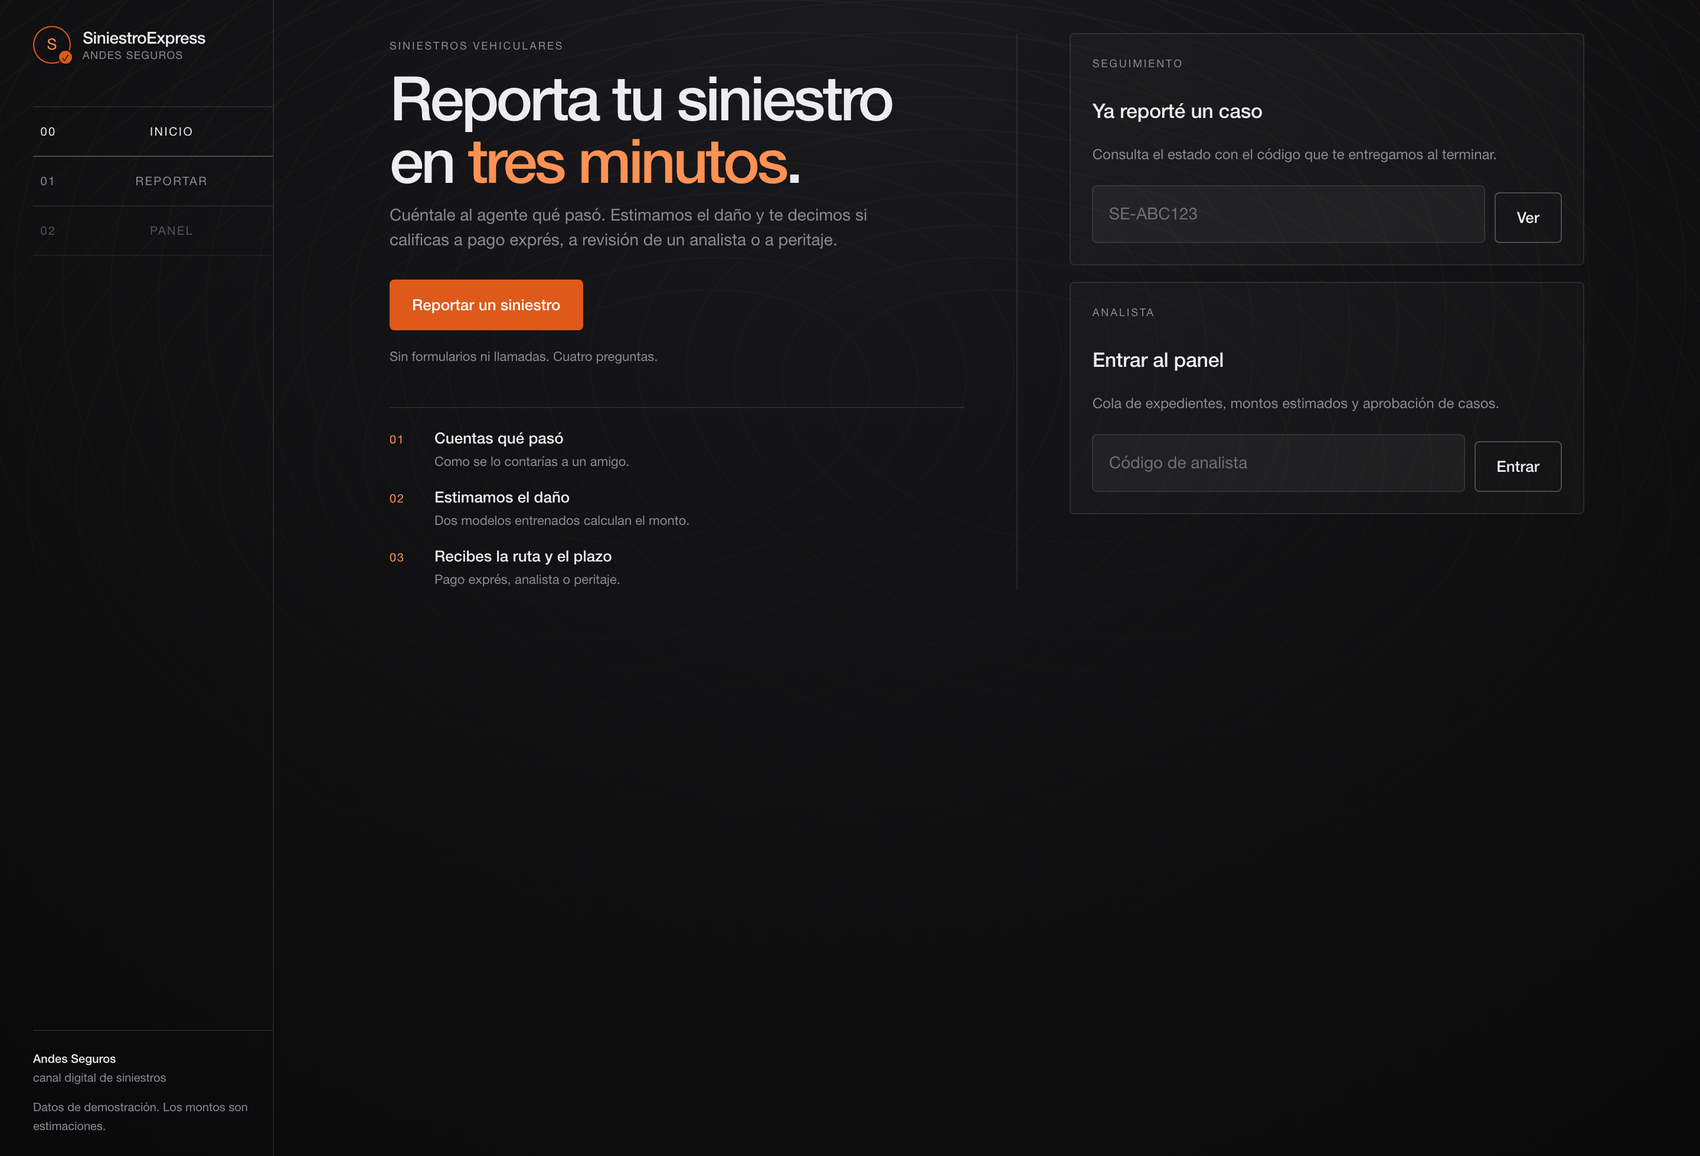
\includegraphics[width=0.78\textwidth]{img/app_inicio.png}
\caption{Pantalla de inicio}
\label{fig:inicio}
\end{figure}

\begin{figure}[htbp]
\centering
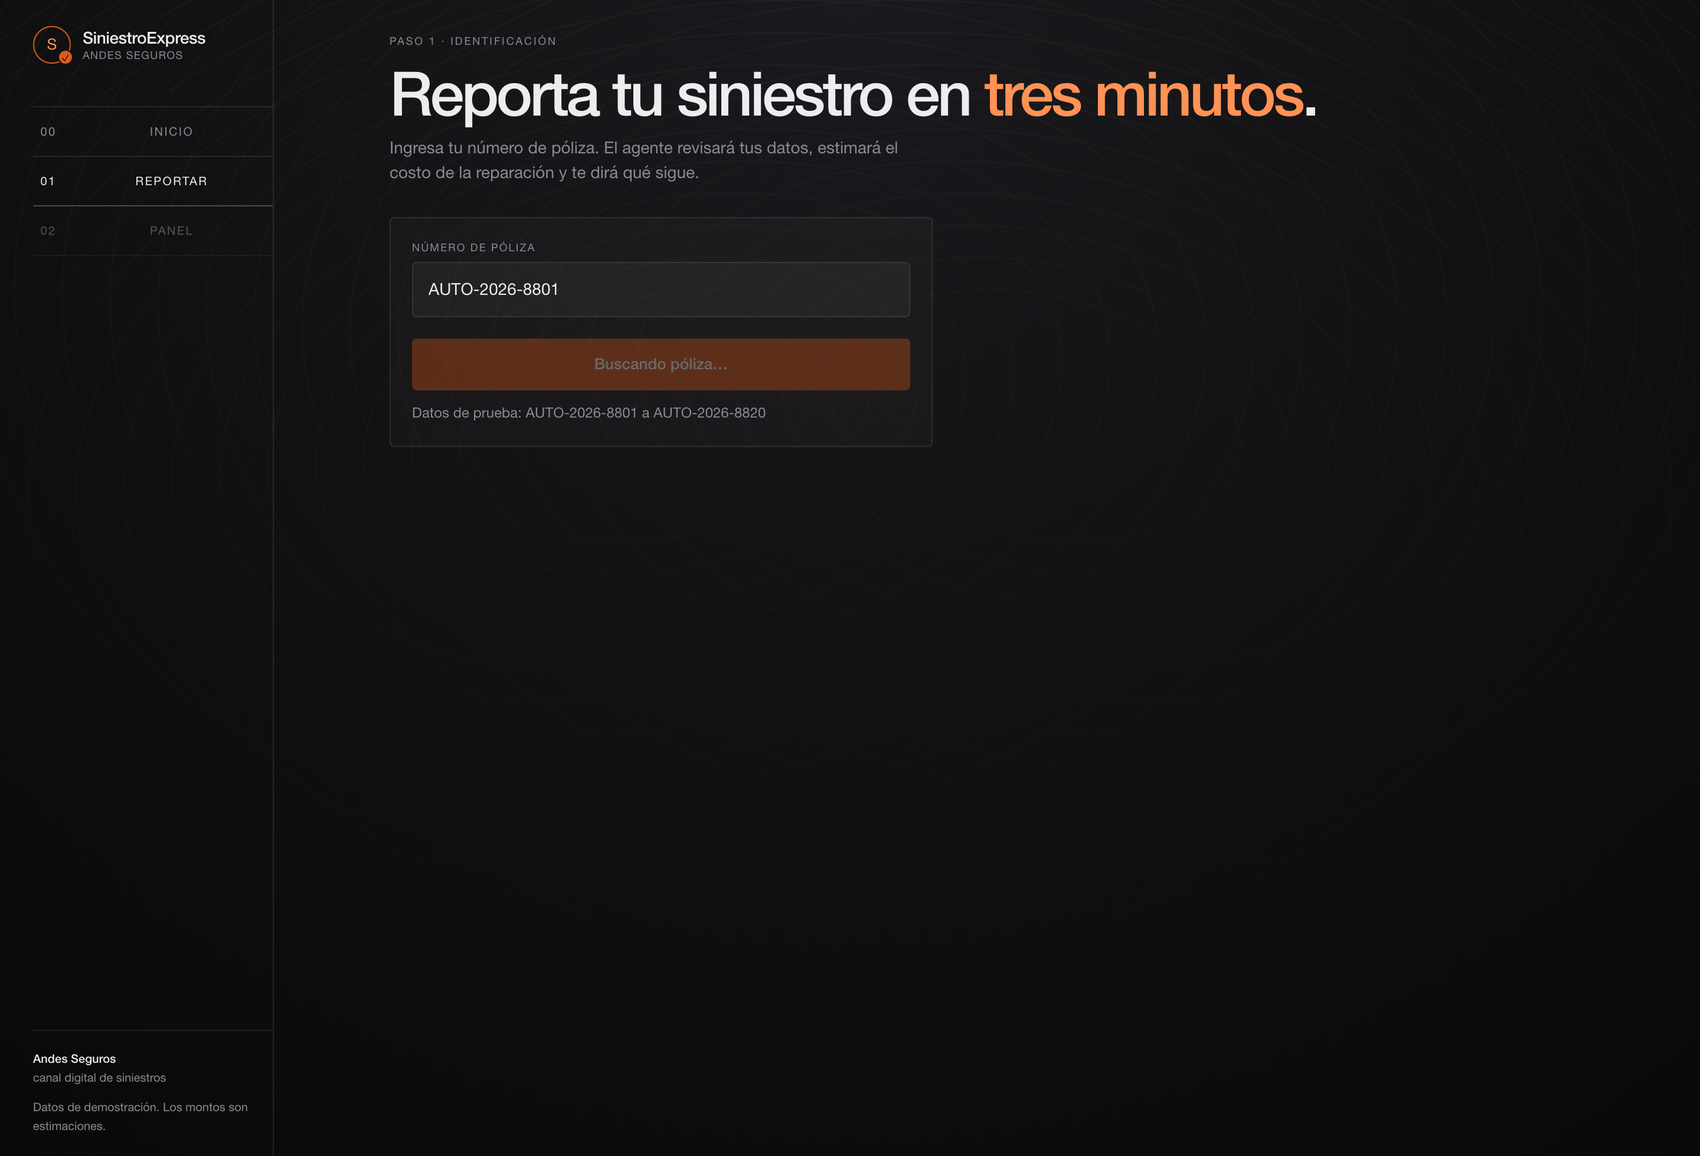
\includegraphics[width=0.8\textwidth]{img/app_chat.png}
\caption{La conversación: el agente saluda, escucha y pregunta lo que falta}
\label{fig:chat}
\end{figure}

\begin{figure}[htbp]
\centering
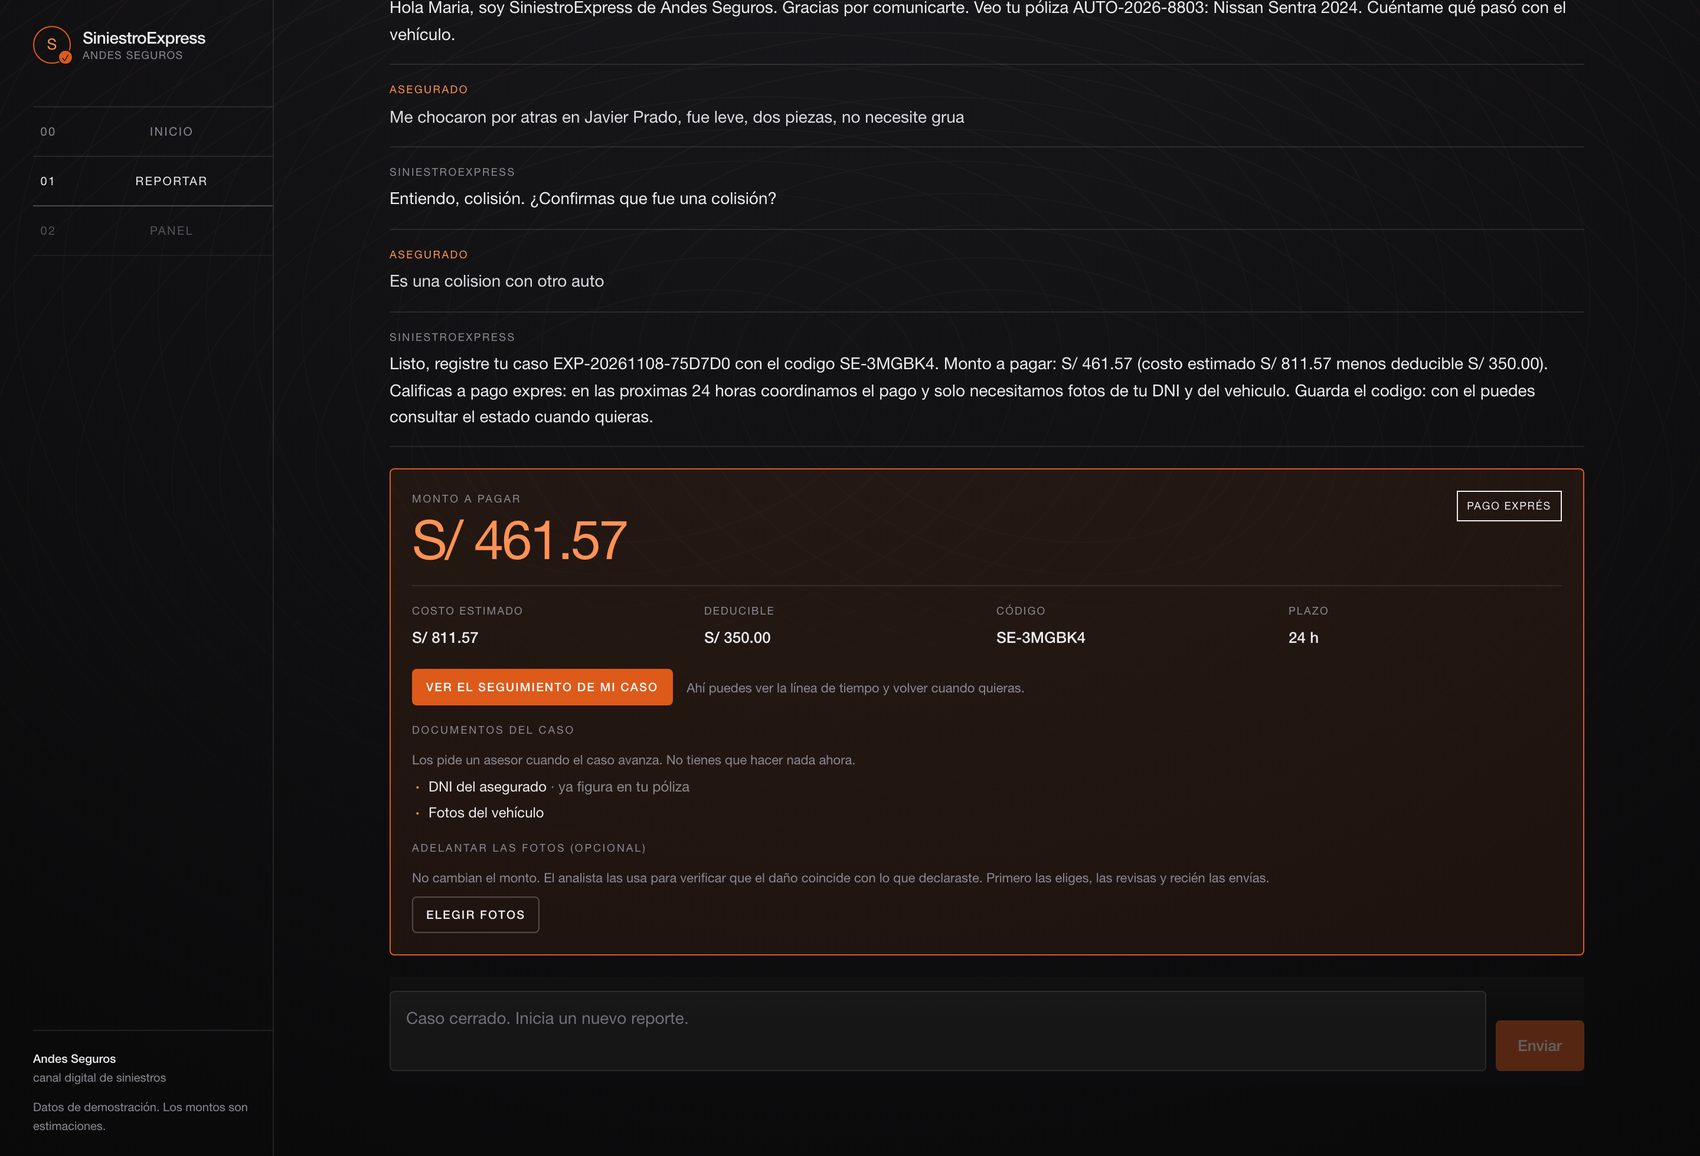
\includegraphics[width=0.8\textwidth]{img/app_veredicto.png}
\caption{Veredicto del caso dentro de la conversación, con su código de seguimiento}
\label{fig:veredicto}
\end{figure}

\begin{figure}[htbp]
\centering
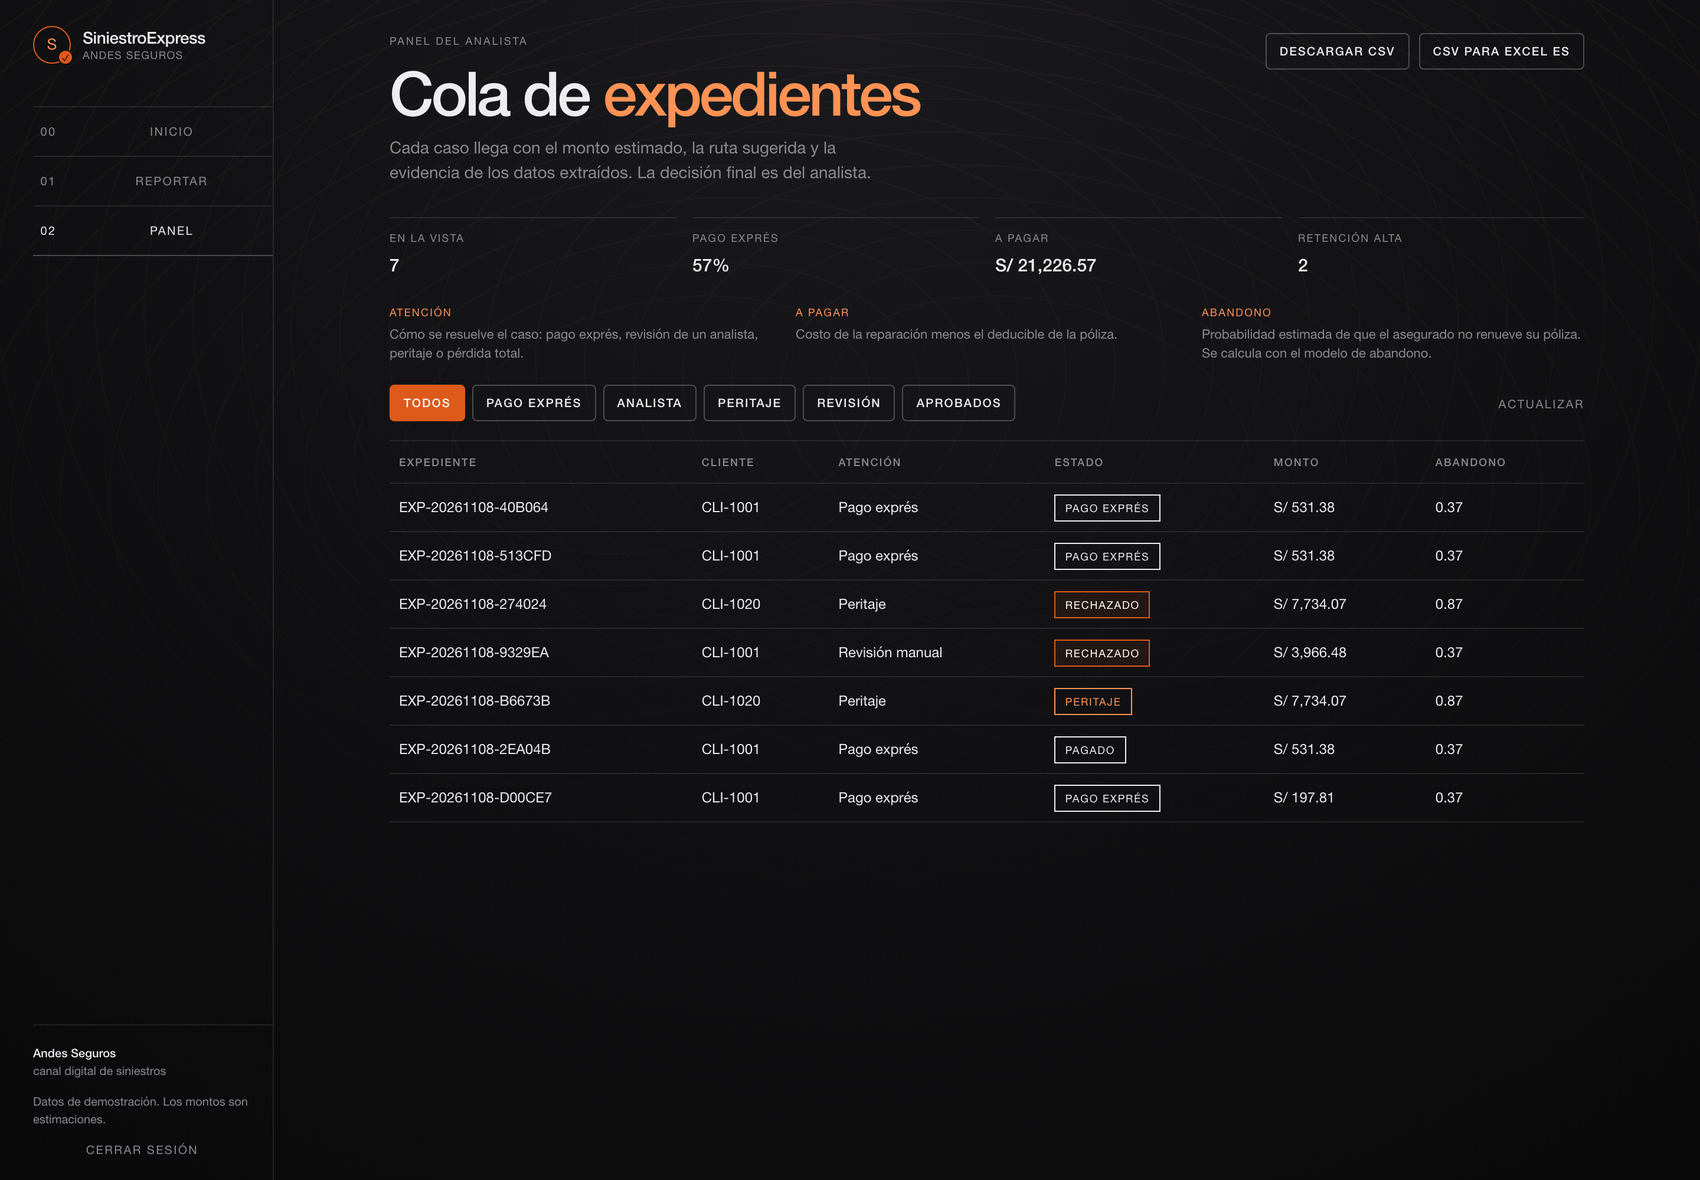
\includegraphics[width=0.8\textwidth]{img/app_panel.png}
\caption{Panel del analista con glosario de términos}
\label{fig:panel}
\end{figure}

\begin{figure}[htbp]
\centering
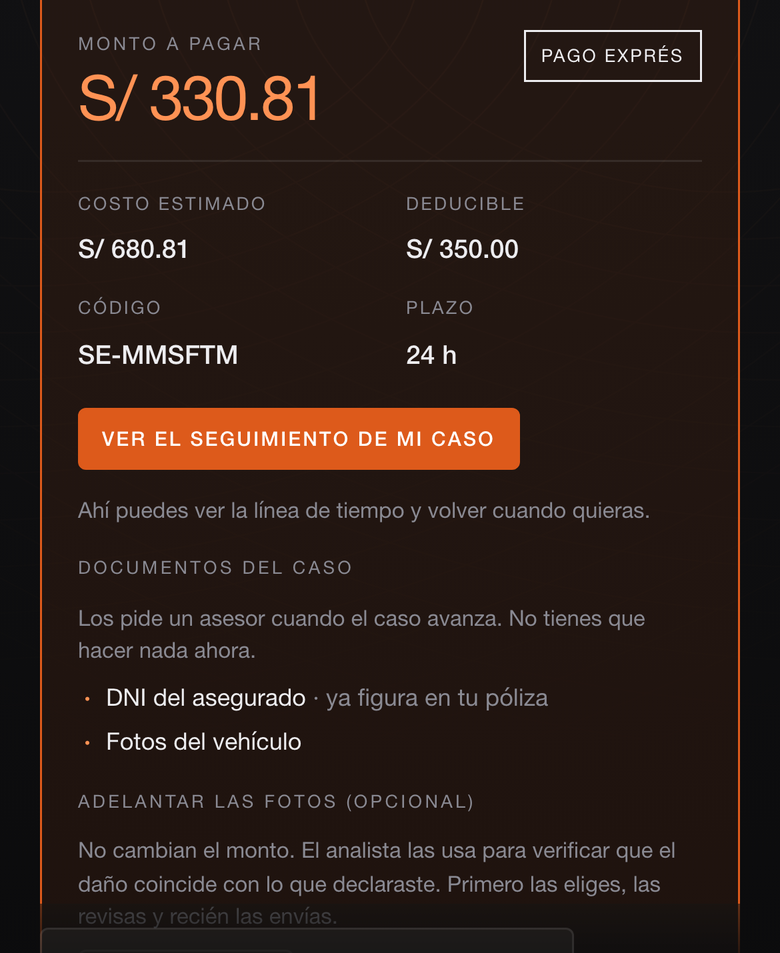
\includegraphics[width=0.46\textwidth]{img/app_movil_chat.png}
\caption{El veredicto en un teléfono: misma información, una sola columna}
\label{fig:movil}
\end{figure}

\subsection{Región elegida y justificación}

La región es \textbf{us-east-1} (Virginia del Norte). La decisión tiene cuatro razones:

\begin{itemize}[itemsep=2pt]
  \item \textbf{Disponibilidad de servicios.} Es la región donde estrenan las
        funcionalidades, lo que reduce el riesgo de que un servicio del proyecto no exista
        todavía en otra zona.
  \item \textbf{Latencia.} Desde Lima, la ida y vuelta ronda los 60 ms, suficiente para
        una conversación por turnos donde el usuario lee la respuesta antes de escribir.
  \item \textbf{Precio.} Es la región con las tarifas más bajas de AWS y donde aplican
        primero las capas gratuitas.
  \item \textbf{Cuenta del laboratorio.} AWS Academy habilita por defecto esa región y
        restringe otras, de modo que elegir otra exigiría permisos adicionales.
\end{itemize}

No se usó una región con presencia local en Perú porque no existe una en el país y porque
la latencia de la conversación no es crítica: el usuario escribe a mano, no compite con un
sistema de tiempo real.

\subsection{Costos y plan de negocio}

\subsubsection{Infraestructura en AWS}

La estimación se hizo en AWS Pricing Calculator con el escenario del piloto: 1,900
siniestros al mes, que generan 20,000 invocaciones de Lambda y 40,000 peticiones a API
Gateway.

\begin{figure}[H]
\centering
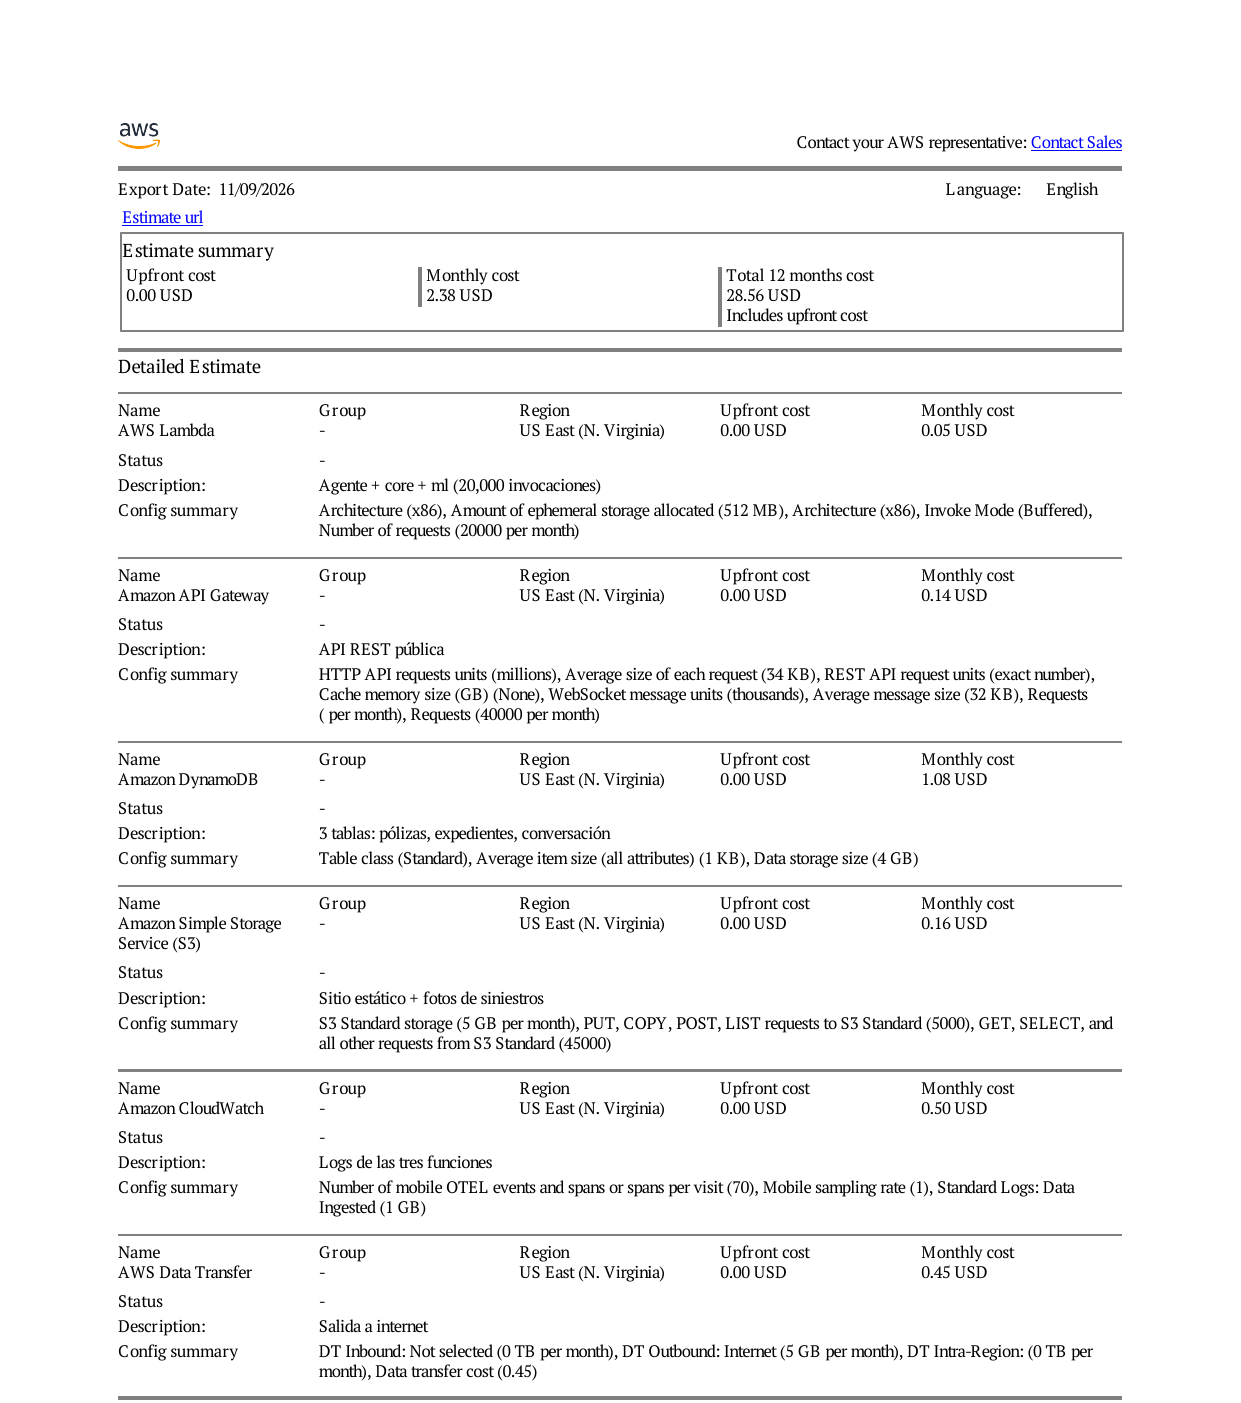
\includegraphics[width=0.58\textwidth]{img/estimate_aws.png}
\caption{Estimación en AWS Pricing Calculator}
\label{fig:calculadora}
\end{figure}

El total es de \textbf{2.38 USD al mes} y 28.56 USD al año, sin costo inicial. La mayor
parte corresponde a DynamoDB (1.08 USD) y a CloudWatch (0.50 USD); Lambda queda en 0.05 USD
porque casi todo el volumen cae dentro de la capa gratuita. El estimado completo está
publicado en
\url{https://calculator.aws/#/estimate?id=e06873a4658ae2ad734f853b9d80956e99e7fbcb}

\subsubsection{El modelo de lenguaje}

El agente usa \code{openai/gpt-oss-120b} a través de la API de Groq, que cobra por token
procesado. Los precios publicados al cierre de este informe son:

\begin{table}[H]
\centering
\caption{Tarifas de Groq para el modelo usado}
\label{tab:groq}
\small
\begin{tabular}{>{\raggedright\arraybackslash}p{5.4cm}>{\raggedright\arraybackslash}p{4.4cm}>{\raggedright\arraybackslash}p{4.6cm}}
\toprule
\textbf{Concepto} & \textbf{Precio por millón de tokens} & \textbf{Equivalente} \\
\midrule
Entrada (texto enviado) & 0.15 USD & 6.7 millones por dólar \\
Entrada en caché & 0.075 USD & 13 millones por dólar \\
Salida (texto generado) & 0.60 USD & 1.7 millones por dólar \\
\bottomrule
\end{tabular}
\end{table}

\begin{figure}[H]
\centering

\includegraphics[width=0.92\textwidth]{img/groq_pricing.png}
\caption{Tarifas publicadas en la página oficial del modelo, en Groq}
\label{fig:groq}
\end{figure}

Una conversación de cinco turnos consume alrededor de 8,000 tokens de entrada, porque el
promedio del sistema y el historial viajan en cada turno, y unos 300 de salida. Con 1,900
casos al mes:

\begin{table}[H]
\centering
\caption{Consumo mensual estimado de Groq}
\label{tab:groq-consumo}
\small
\begin{tabular}{>{\raggedright\arraybackslash}p{5.2cm}>{\raggedright\arraybackslash}p{3.6cm}>{\raggedright\arraybackslash}p{3.4cm}>{\raggedright\arraybackslash}p{2.4cm}}
\toprule
\textbf{Concepto} & \textbf{Tokens al mes} & \textbf{Precio unitario} & \textbf{Costo} \\
\midrule
Entrada & 15.2 millones & 0.15 USD / M & 2.28 USD \\
Salida & 0.57 millones & 0.60 USD / M & 0.34 USD \\
\midrule
\textbf{Total} & & & \textbf{2.62 USD} \\
\bottomrule
\end{tabular}
\end{table}

\subsubsection{El plan para Andes Seguros}

Sumando las dos piezas, operar el sistema cuesta \textbf{5.00 USD al mes} para 1,900 casos:
menos de tres décimos de centavo por siniestro. Sobre esa base se proponen dos
suscripciones, y el precio no se fija sobre el costo de la infraestructura, que es
simbólico, sino sobre el tiempo administrativo que el servicio absorbe.

\begin{table}[H]
\centering
\caption{Suscripciones propuestas}
\label{tab:plan}
\small
\sloppy
\begin{tabular}{>{\raggedright\arraybackslash}p{3.4cm}>{\raggedright\arraybackslash}p{2.6cm}>{\raggedright\arraybackslash}p{2.6cm}>{\raggedright\arraybackslash}p{3.2cm}>{\raggedright\arraybackslash}p{3.0cm}}
\toprule
\textbf{Plan} & \textbf{Precio} & \textbf{Casos al mes} & \textbf{Costo estimado} & \textbf{Margen} \\
\midrule
Básico & 20 USD & hasta 5,000 & 13.16 USD & 6.84 USD (34 \%) \\
Escala & 100 USD & hasta 25,000 & 65.80 USD & 34.20 USD (34 \%) \\
\bottomrule
\end{tabular}
\end{table}

El costo estimado se calculó escalando el piloto de forma lineal, que es un techo
conservador: DynamoDB no crece con el número de casos sino con el almacenamiento, y Lambda
y API Gateway tienen capas gratuitas que absorben el primer tramo. A 5,000 casos, Groq
consume 6.90 USD y AWS unos 6.26 USD; a 25,000, la proporción se mantiene.

La lógica comercial es simple. El plan Básico cubre el doble del piloto y deja un margen
del 34 \%, que alcanza para operar y sostener el soporte. El plan Escala cuesta cinco veces
más porque atiende cinco veces más casos, pero el margen porcentual no cambia: el servicio
no gana por volumen, gana porque reemplaza trabajo repetitivo.

El punto de equilibrio del cliente es inmediato: con un solo caso que evite media hora de
trabajo administrativo, la suscripción del mes ya se pagó. Y para el proveedor también:
con 1,900 casos, el costo de operación son 5.00 USD sobre una suscripción de 20.00 USD.

\clearpage
\section{Parte C: implementación}

\subsection{Estructura del repositorio}

El repositorio \code{github.com/UTEC-AII/siniestro-express} está organizado por servicio y
por etapa del pipeline.

\begin{table}[H]
\centering
\caption{Organización del repositorio}
\label{tab:repo}
\small
\begin{tabular}{p{4.2cm}p{8.4cm}}
\toprule
\textbf{Carpeta} & \textbf{Contenido} \\
\midrule
\code{services/agente} & Chat con memoria, normalización de slots, prompt y cliente de Groq \\
\code{services/core} & Pólizas, expedientes, liquidación, estados, fotos y exportación \\
\code{services/ml} & Modelos exportados, runtime de inferencia y API de predicción \\
\code{services/ml/training} & Datos, fórmula de costos, entrenamiento y verificación de paridad \\
\code{frontend} & Aplicación React con Vite, cuatro vistas y despliegue a S3 \\
\code{seed} & 20 pólizas de prueba y scripts de carga y reinicio \\
\code{docs} & Arquitectura, runbook, capturas, colección de Postman y notas de dependencias \\
\code{tests} & Pruebas de integración con DynamoDB simulado \\
\bottomrule
\end{tabular}
\end{table}

\subsection{Despliegue}

El procedimiento completo está en \code{docs/runbook-despliegue.md} del repositorio. Se
ejecuta sobre la instancia de desarrollo de AWS Academy, que es una máquina Ubuntu con
CloudShell, y sigue este orden:

\begin{enumerate}[itemsep=2pt]
  \item \textbf{Preparar la máquina.} Node.js 20.19 o superior, Serverless Framework v4 y
        \code{boto3} para los scripts de carga. Las tres cosas se instalan una sola vez.
  \item \textbf{Renovar las credenciales.} AWS Academy las entrega por cuatro horas y hay
        que pegarlas en \code{~/.aws/credentials} al empezar cada sesión.
  \item \textbf{Fijar la región.} \code{aws configure set region us-east-1} escribe en
        \code{~/.aws/config}. Va ahí y no en el archivo de credenciales, porque ese se
        reescribe cada cuatro horas y se llevaría la región por delante.
  \item \textbf{Clonar el repositorio} en \code{/home/ubuntu} y entrar a la carpeta.
  \item \textbf{Definir las cinco variables} en un archivo \code{.env}: la clave de Groq,
        las tres URL de API Gateway y la del servicio core para el frontend. Los
        \code{serverless.yml} las leen al empaquetar, y si falta una el despliegue se cae
        con un error que no dice cuál.
  \item \textbf{Desplegar en orden.} Primero \code{ml}, que no necesita nada y devuelve su
        URL; después \code{core}, que necesita la de \code{ml}; y al final \code{agente},
        que necesita la de \code{core}. Cada despliegue imprime sus endpoints.
  \item \textbf{Sembrar las pólizas} con \code{python3 seed/seed.py}. El script valida los
        quince campos de cada póliza antes de escribirla.
  \item \textbf{Publicar el frontend} con \code{./scripts/deploy.sh web}. Vite incrusta las
        dos URL en el paquete, así que hay que compilar después de conocerlas.
  \item \textbf{Comprobar.} \code{curl} a \code{/ml/health} y un \code{POST} a
        \code{/expedientes} confirman que los tres servicios se hablan entre sí.
  \item \textbf{Redesplegar solo lo que cambió.} Si se toca el prompt, va \code{agente};
        si cambian las reglas, \code{core}; si cambian los modelos, \code{ml}.
\end{enumerate}

El script \code{scripts/deploy.sh} envuelve los pasos 5 y 6: verifica que las variables
existan antes de llamar a Serverless, para no perder tiempo en un empaquetado que va a
fallar. Las URL de cada servicio, una vez desplegados, quedan como \emph{Output} del stack
de CloudFormation, de modo que se pueden recuperar aunque se pierda la sesión.

\subsection{Evidencias con Postman}

La colección tiene 19 peticiones en cinco carpetas y cada una incluye pruebas automáticas.
Se ejecuta de arriba hacia abajo: las variables se encadenan solas, porque cada petición
guarda lo que la siguiente necesita.

\begin{figure}[htbp]
\centering
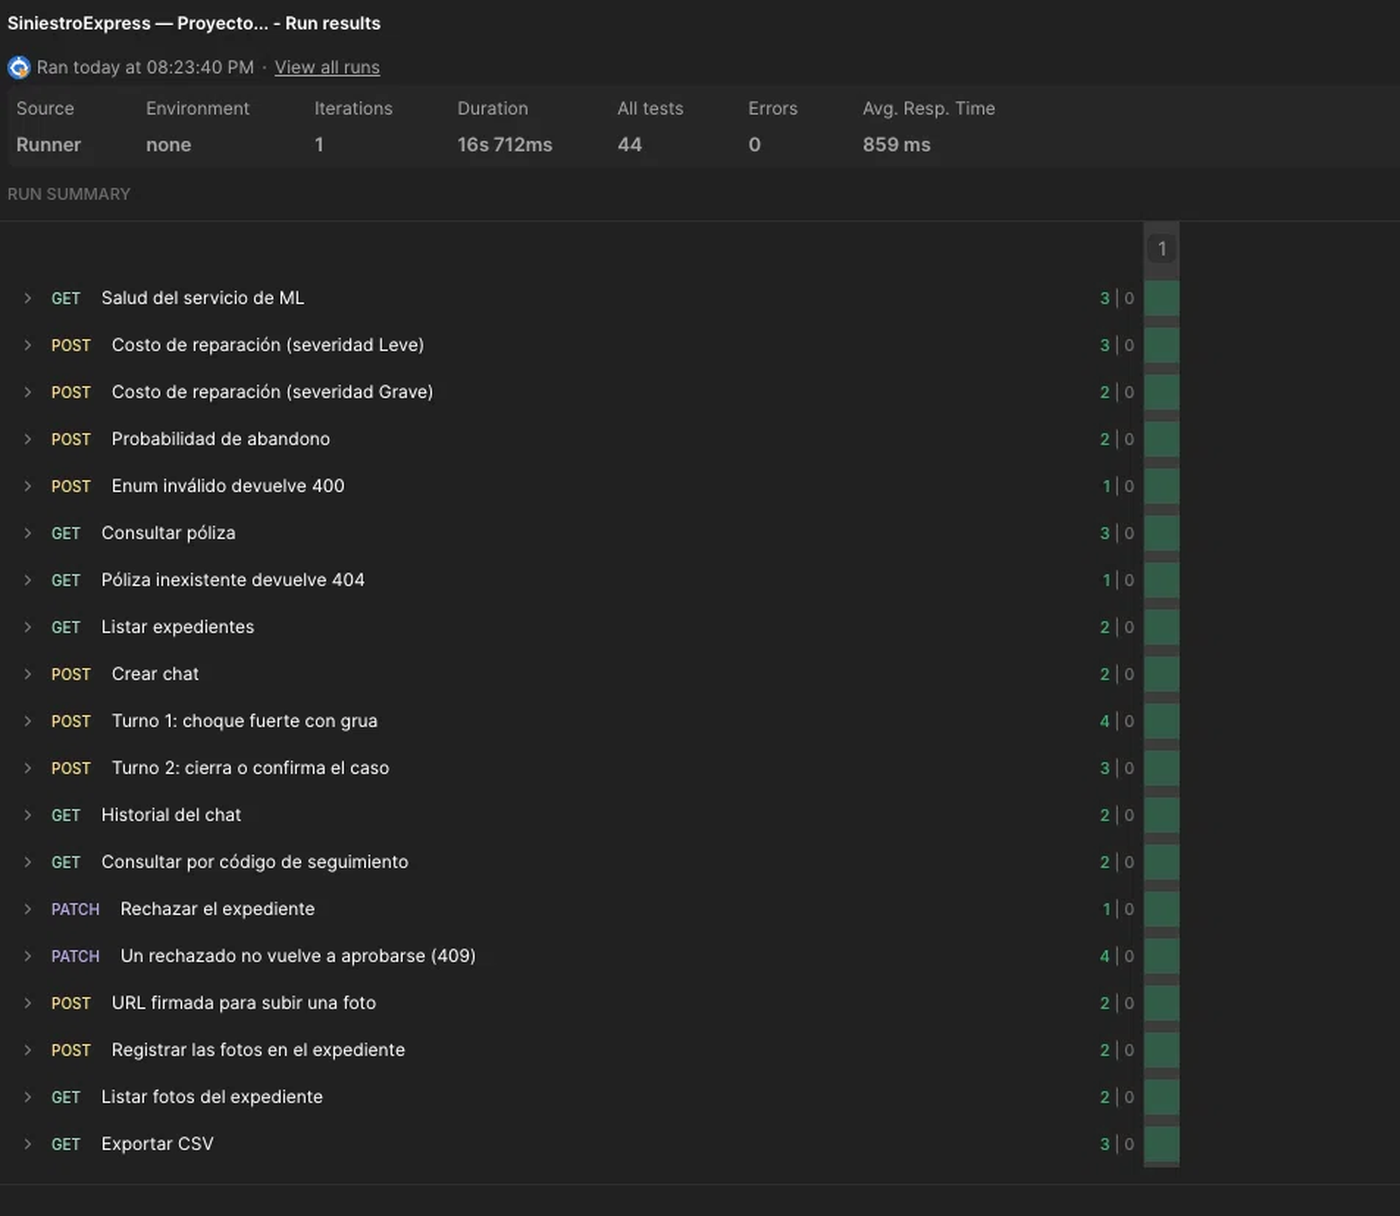
\includegraphics[width=0.44\textwidth]{img/postman_runner.png}
\caption{Corrida completa de la colección: 19 peticiones, 44 pruebas, 0 fallos}
\label{fig:runner}
\end{figure}

La corrida completa es la evidencia más compacta del backend: las 19 peticiones se
ejecutan en cadena y las \textbf{44 pruebas} pasan sin un solo fallo, en 16,7 segundos. La
colección se diseñó para que cada petición deje listo lo que la siguiente necesita, de modo
que una corrida limpia demuestra el flujo entero y no una suma de casos aislados.

\begin{table}[H]
\centering
\caption{Origen de las 44 pruebas de la corrida}
\label{tab:pruebas-postman}
\footnotesize
\sloppy
\begin{tabular}{>{\raggedright\arraybackslash}p{6.0cm}>{\centering\arraybackslash}p{1.5cm}>{\raggedright\arraybackslash}p{6.9cm}}
\toprule
\textbf{Petición} & \textbf{Pruebas} & \textbf{Qué comprueba} \\
\midrule
Salud del servicio de ML & 3 & Los dos modelos cargados, 250 y 200 árboles \\
Costo de reparación, Leve & 3 & Estado, moneda y que el monto no pase el umbral de pago exprés \\
Costo de reparación, Grave & 2 & Estado y que el monto suba con la severidad \\
Probabilidad de abandono & 2 & Estado y probabilidad entre 0 y 1 \\
Enum inválido & 1 & El 400 por un valor fuera del catálogo \\
Consultar póliza & 3 & Estado, vehículo y deducible de la póliza \\
Póliza inexistente & 1 & El 404 con un identificador que no existe \\
Listar expedientes & 2 & Estado y que la respuesta sea una lista \\
Crear chat & 2 & Estado 201 y la forma del identificador \\
Turno 1 & 4 & Estado, piezas, grúa y tipo de siniestro \\
Turno 2 & 3 & Expediente creado, formato del código y liquidación \\
Historial del chat & 2 & Estado y que la conversación se conserve \\
Consultar por código & 2 & Estado y presencia de la ruta asignada \\
Rechazar el expediente & 1 & El cambio de estado permitido \\
Un rechazado no se aprueba & 4 & El 409 y el estado actual en el cuerpo \\
URL firmada & 2 & El enlace de subida y la clave del objeto \\
Registrar las fotos & 2 & Estado y conteo de fotos registradas \\
Listar fotos & 2 & Estado y que devuelva la lista \\
Exportar CSV & 3 & Estado, tipo de contenido y separador \\
\midrule
\textbf{Total} & \textbf{44} & \\
\bottomrule
\end{tabular}
\end{table}

Las pruebas no se limitan a comprobar que la respuesta sea 200. Cada una verifica
\textbf{contratos}: que el código de seguimiento tenga el formato esperado, que el monto a
pagar sea menor que el costo, que la probabilidad esté entre 0 y 1, y que los tres casos que
deben fallar devuelvan el código HTTP correcto con su explicación en el cuerpo.

El promedio de 859 ms por petición lo dominan las dos llamadas al modelo de lenguaje, que
tardan alrededor de cinco segundos cada una; el resto responde en decenas de milisegundos.
Es el comportamiento esperado cuando la latencia la fija el proveedor del modelo y no la
infraestructura propia.

\begin{figure}[H]
\centering
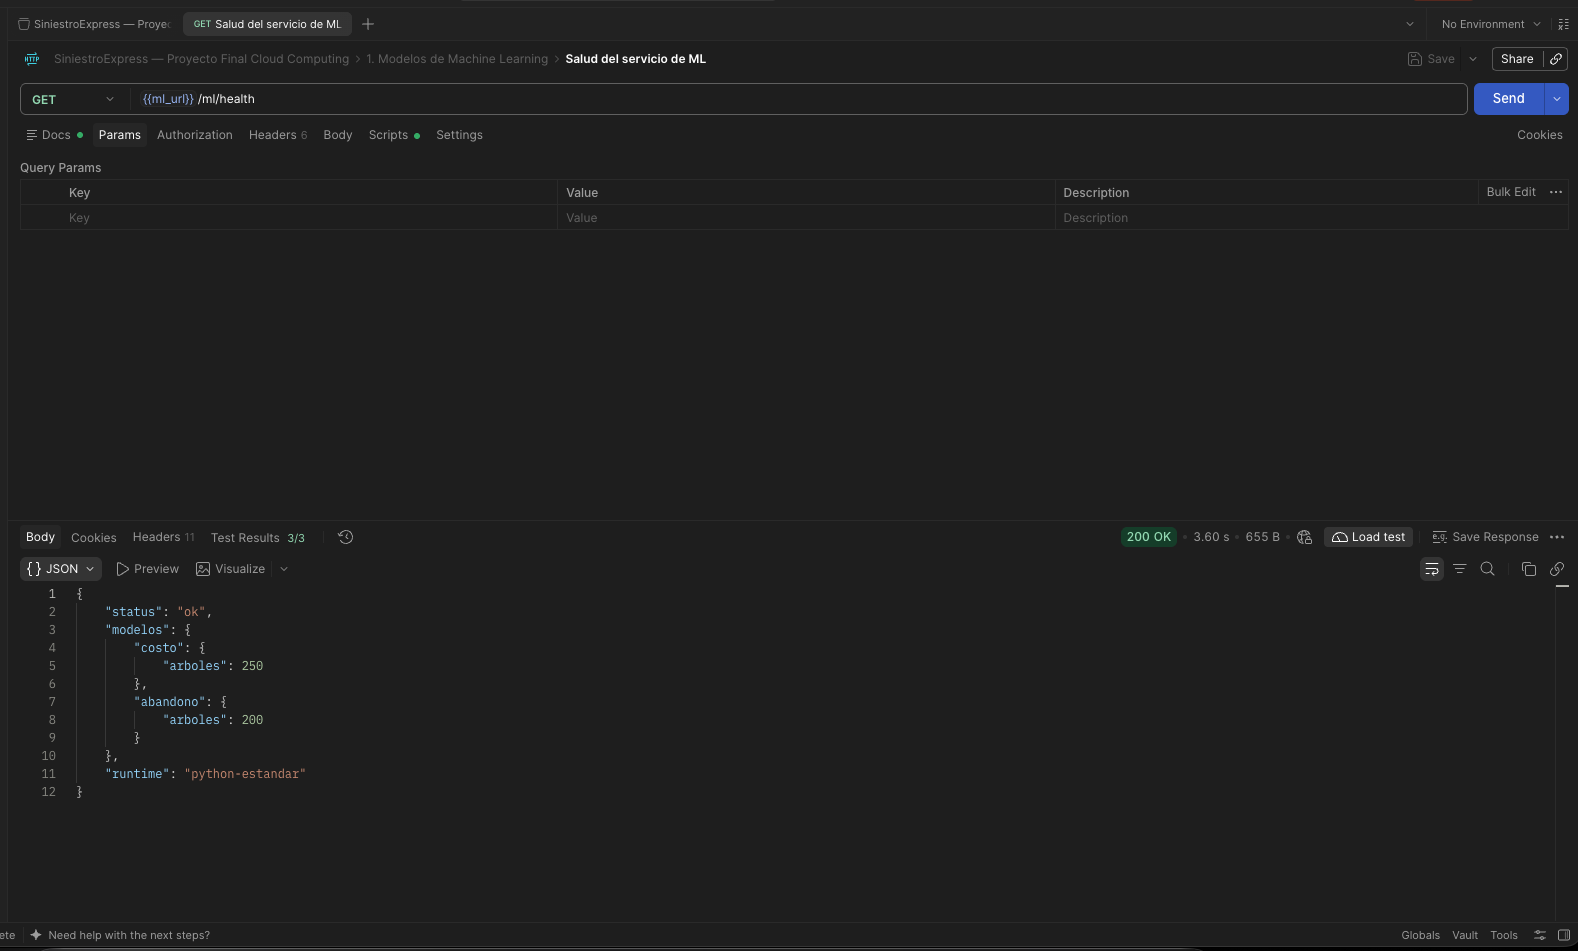
\includegraphics[width=0.95\textwidth]{img/postman_coleccion.png}
\caption{Colección importada y verificación del servicio de modelos}
\label{fig:p1}
\end{figure}

\begin{figure}[H]
\centering
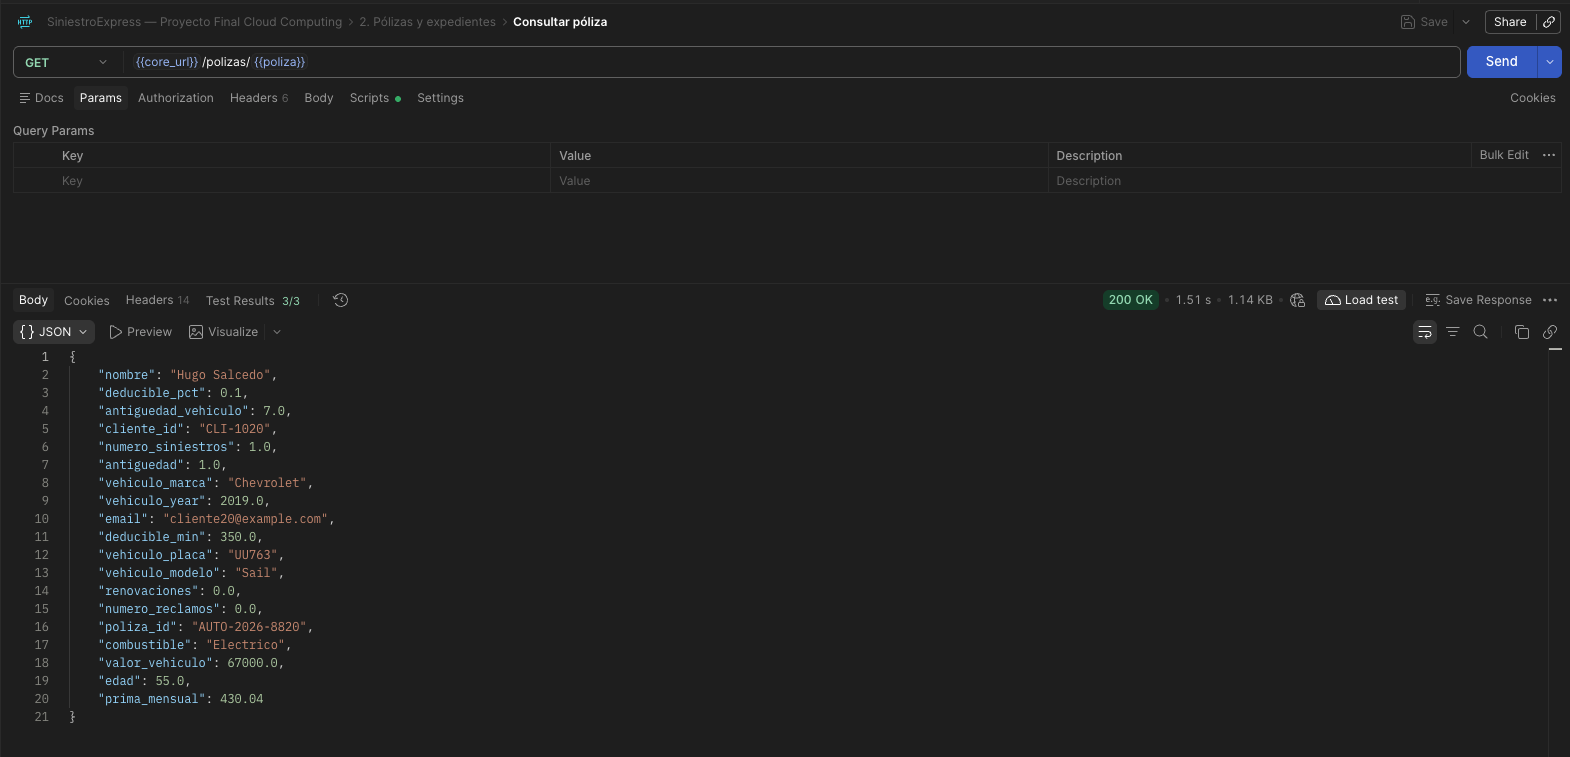
\includegraphics[width=0.95\textwidth]{img/postman_poliza.png}
\caption{Consulta de póliza con vehículo y deducible}
\label{fig:p2}
\end{figure}

\begin{figure}[H]
\centering
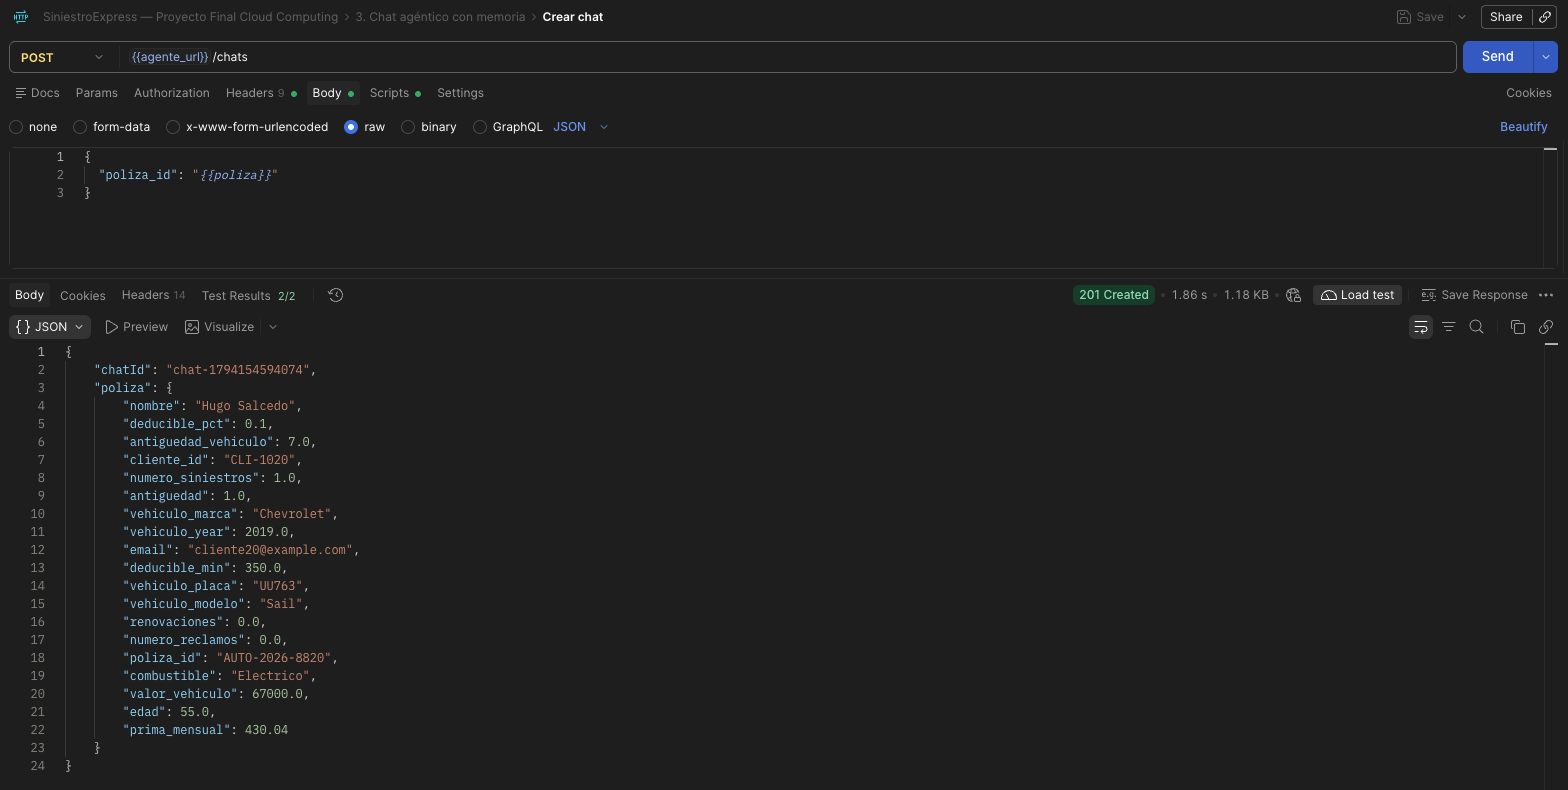
\includegraphics[width=0.95\textwidth]{img/postman_chat.png}
\caption{Creación de la conversación: el cuerpo usa la variable de la póliza}
\label{fig:p3}
\end{figure}

\begin{figure}[H]
\centering
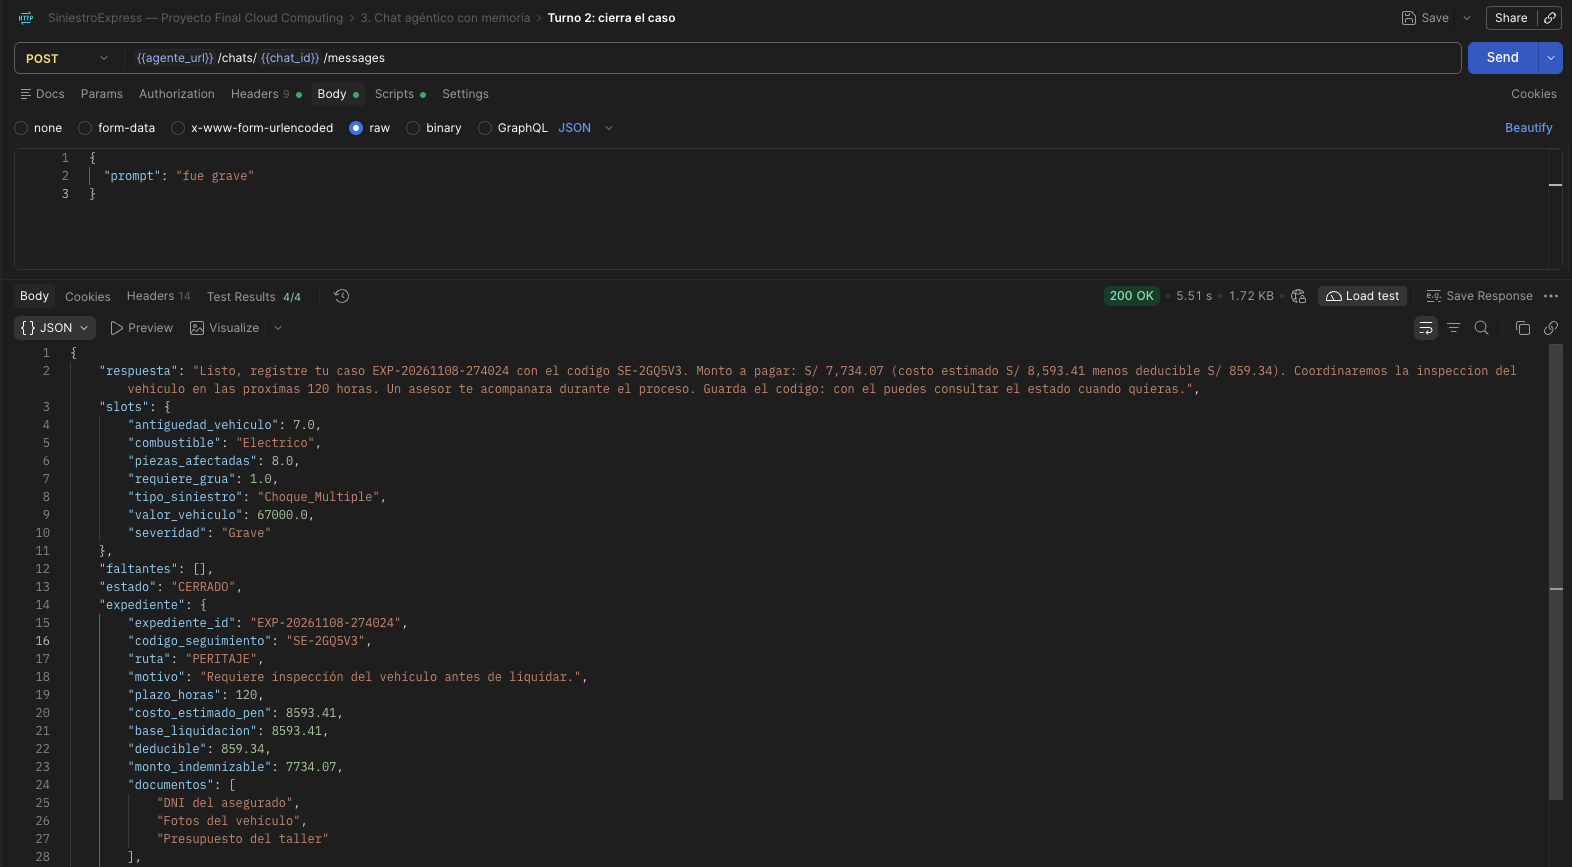
\includegraphics[width=0.95\textwidth]{img/postman_turno2.png}
\caption{Segundo turno: el expediente queda creado con su código y su liquidación}
\label{fig:p4}
\end{figure}

\begin{figure}[H]
\centering
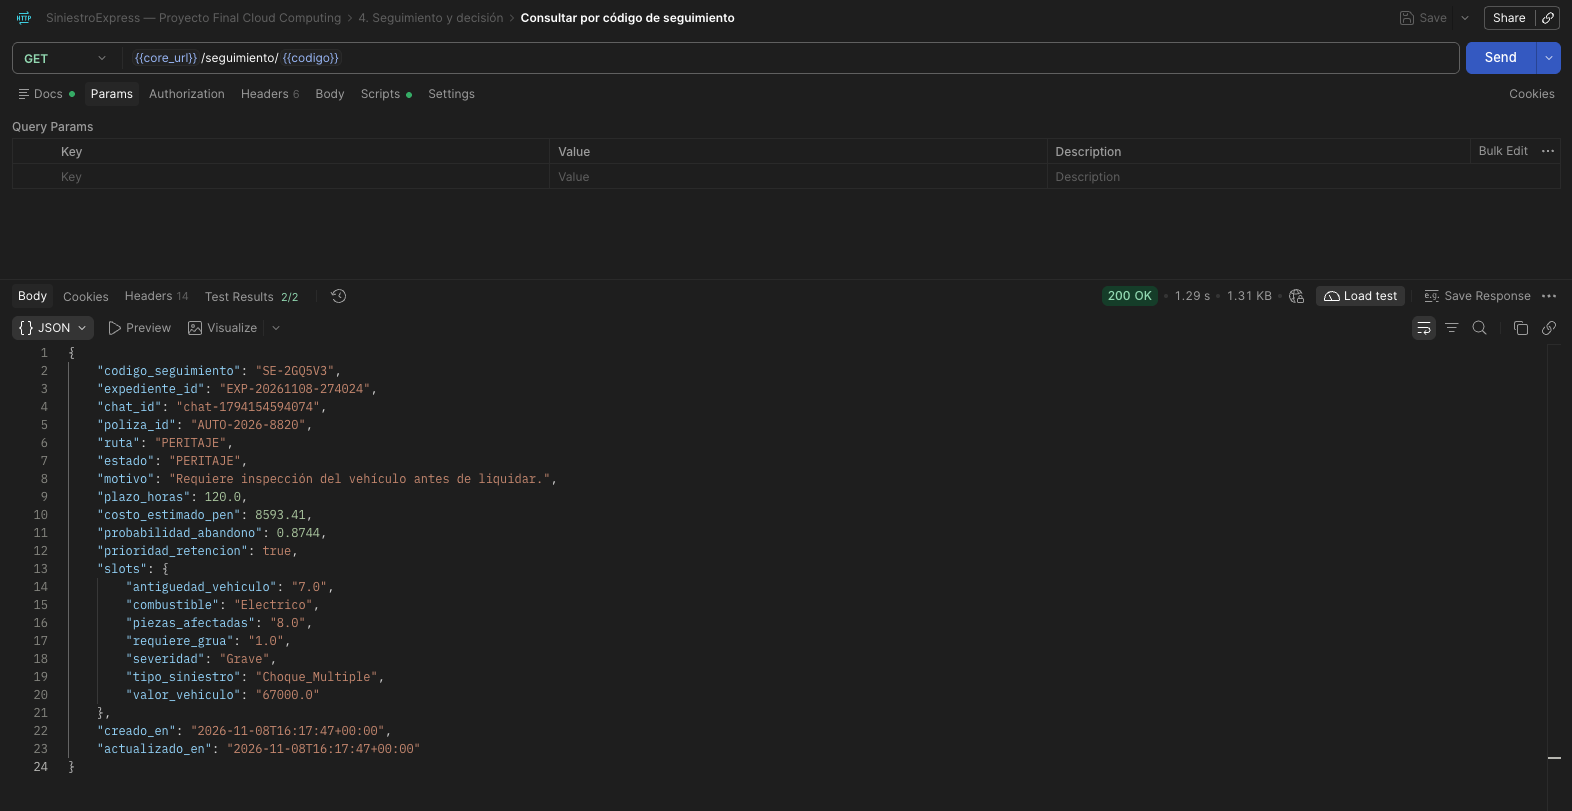
\includegraphics[width=0.95\textwidth]{img/postman_seguimiento.png}
\caption{Consulta por código de seguimiento}
\label{fig:p5}
\end{figure}

\begin{figure}[H]
\centering
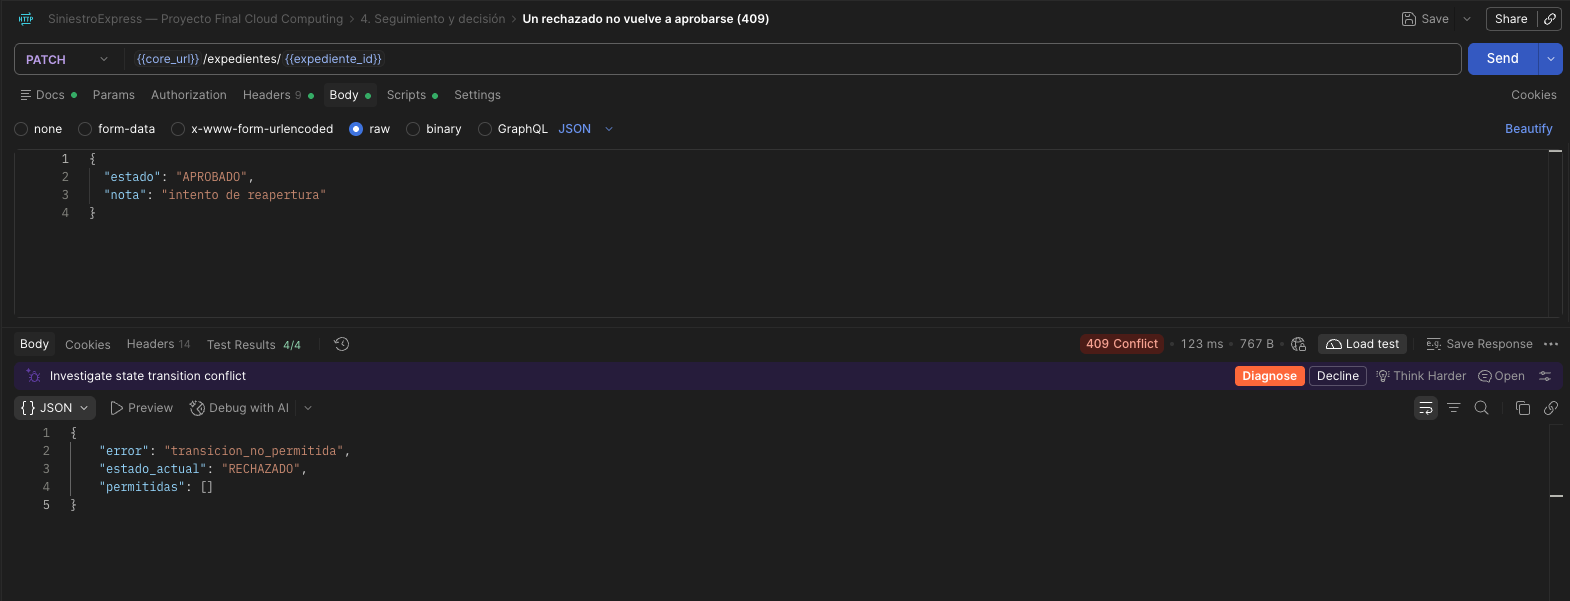
\includegraphics[width=0.95\textwidth]{img/postman_409.png}
\caption{Rechazo de una transición no permitida}
\label{fig:p6}
\end{figure}

\begin{figure}[H]
\centering
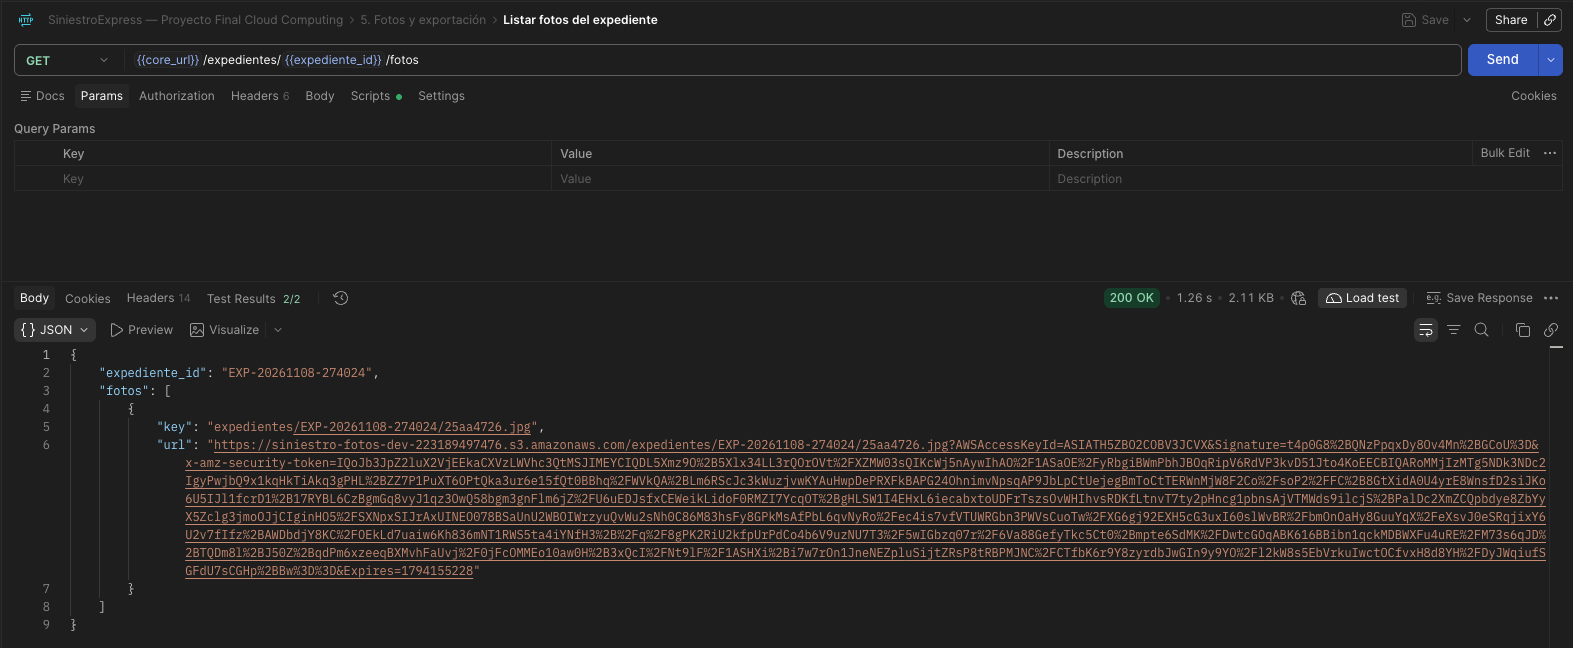
\includegraphics[width=0.95\textwidth]{img/postman_fotos.png}
\caption{Listado de fotos con URL firmadas}
\label{fig:p7}
\end{figure}

\begin{figure}[H]
\centering
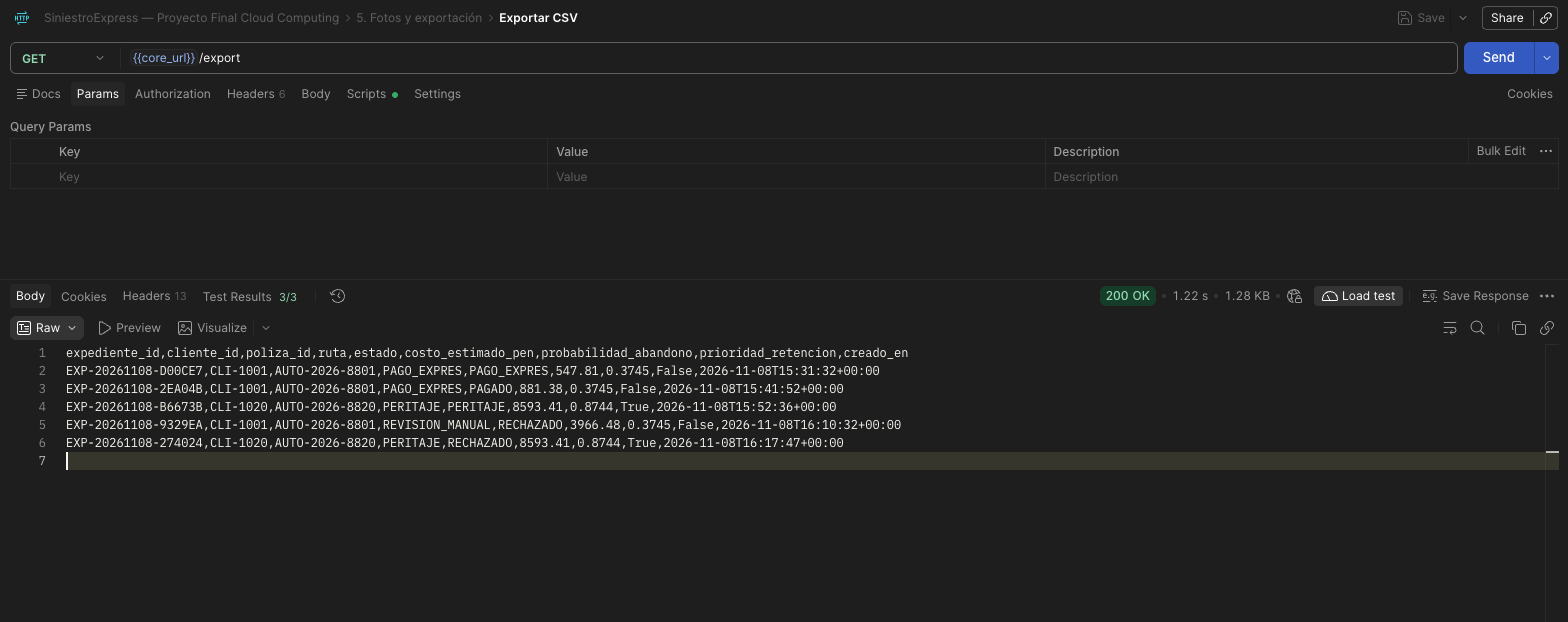
\includegraphics[width=0.95\textwidth]{img/postman_csv.png}
\caption{Exportación del CSV de expedientes}
\label{fig:p8}
\end{figure}

La captura de la consulta por código es la que mejor resume el sistema: en una sola
respuesta aparecen el código, el expediente, la póliza, la ruta, el estado, el motivo, el
plazo, el costo estimado, la probabilidad de abandono y los siete datos extraídos de la
conversación.

\subsection{Evidencias en la consola de AWS}

El despliegue dejó los recursos con la forma descrita, y las tres consolas lo confirman. Lambda
muestra las 17 funciones del proyecto en Python 3.14, empaquetadas en Zip y nombradas por
servicio y etapa. DynamoDB muestra las tres tablas con sus claves de partición y el número
de índices secundarios de cada una. S3 muestra los dos buckets: el del sitio web y el de
las fotos.


\begin{figure}[H]
\centering
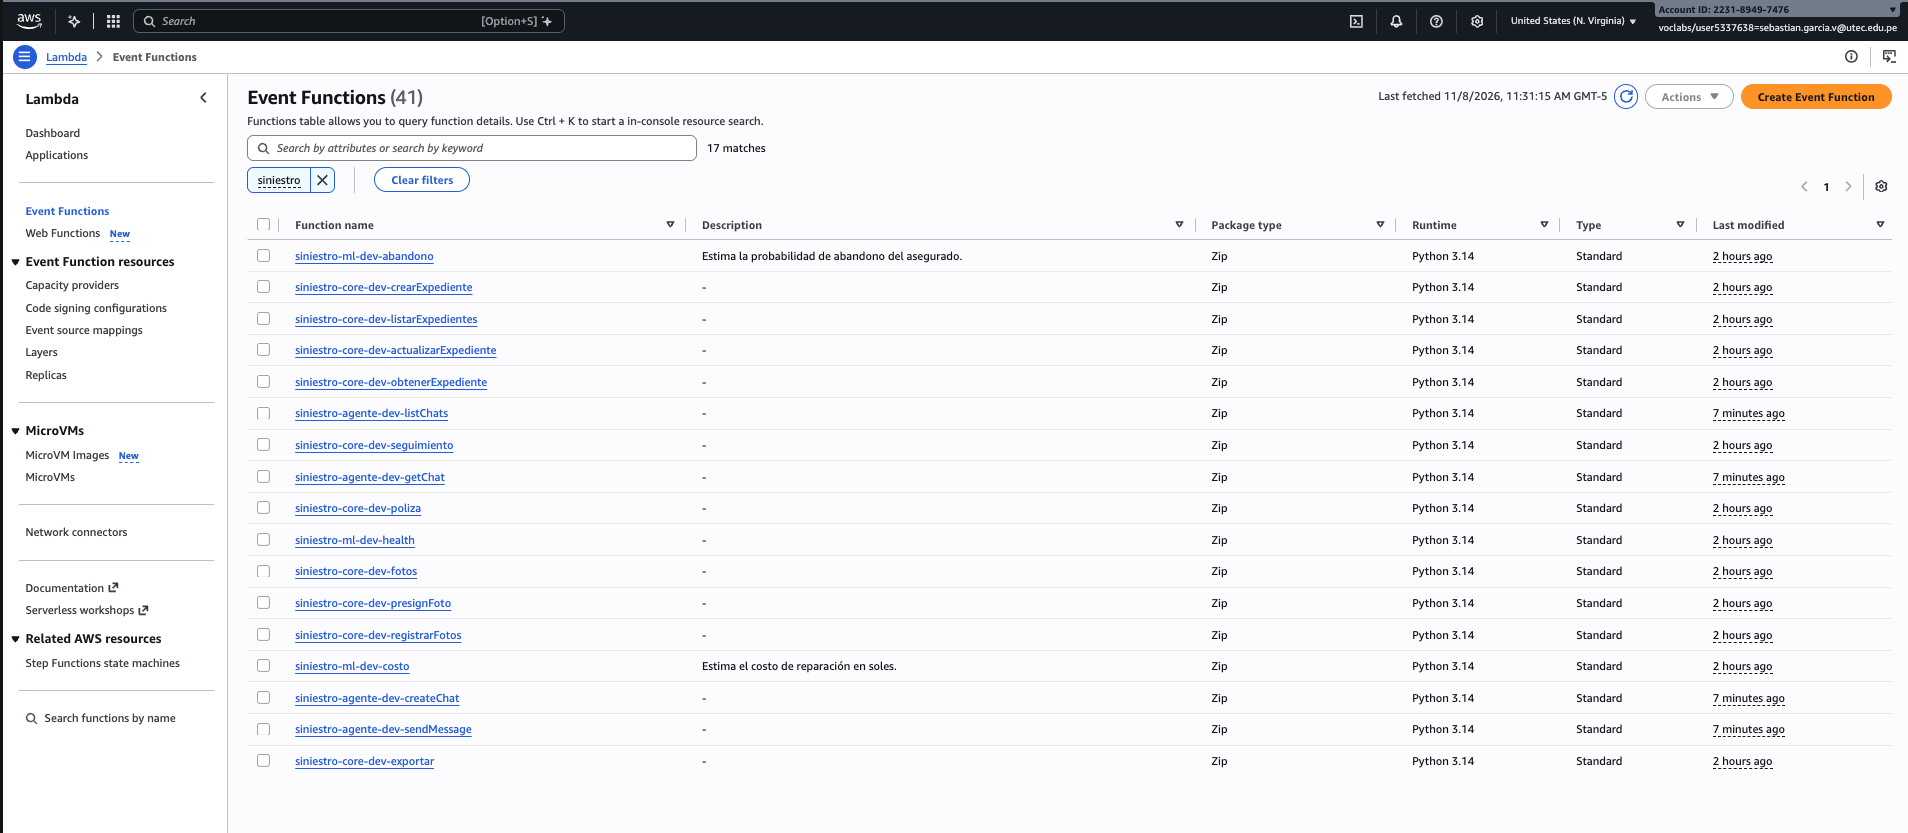
\includegraphics[width=0.95\textwidth]{img/aws_lambda.png}
\caption{Las 17 funciones Lambda del proyecto}
\label{fig:lambda}
\end{figure}

\begin{figure}[H]
\centering
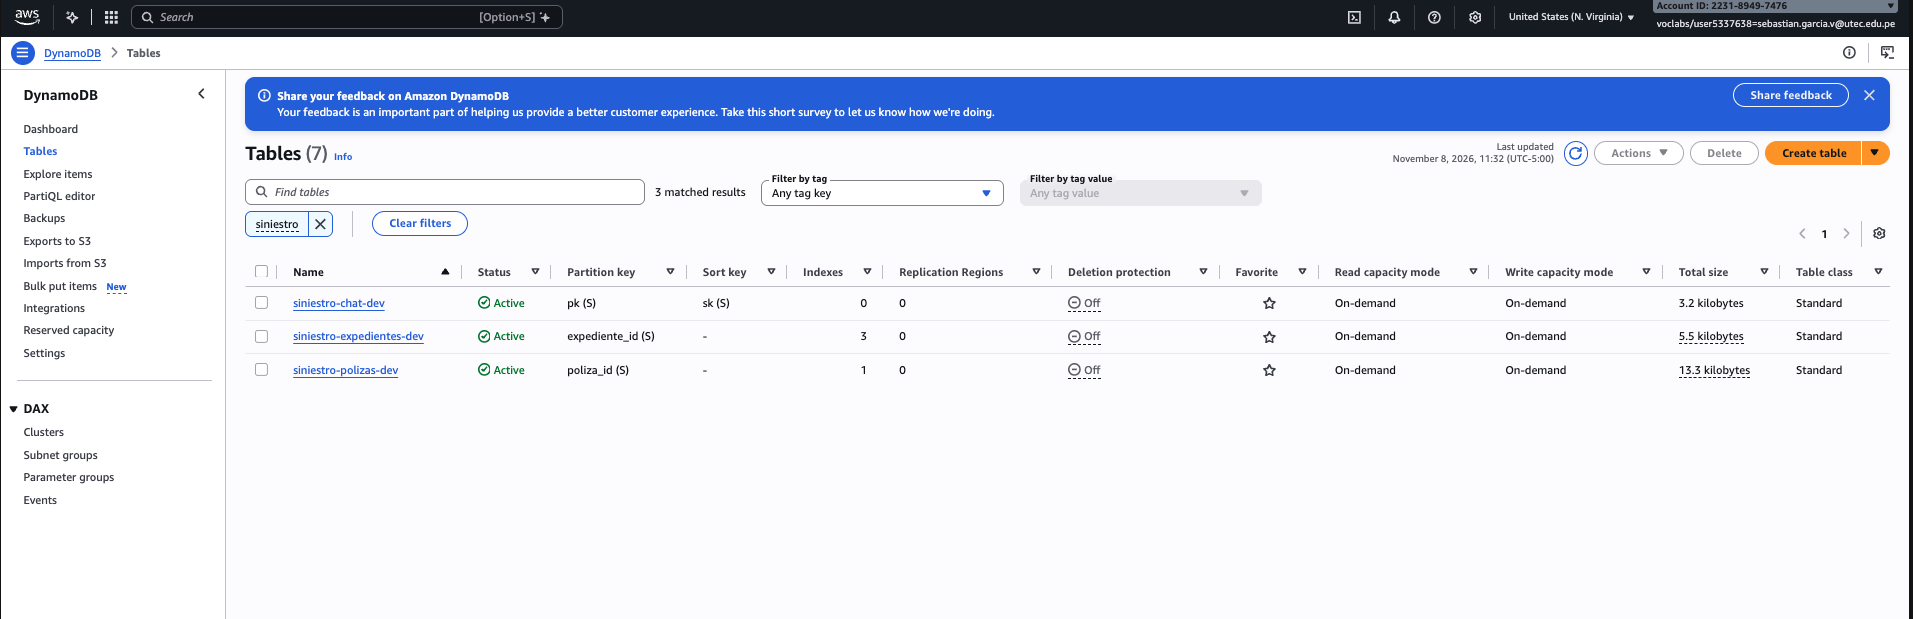
\includegraphics[width=0.95\textwidth]{img/aws_dynamodb.png}
\caption{Las tres tablas de DynamoDB con sus índices}
\label{fig:dynamodb}
\end{figure}

\begin{figure}[H]
\centering
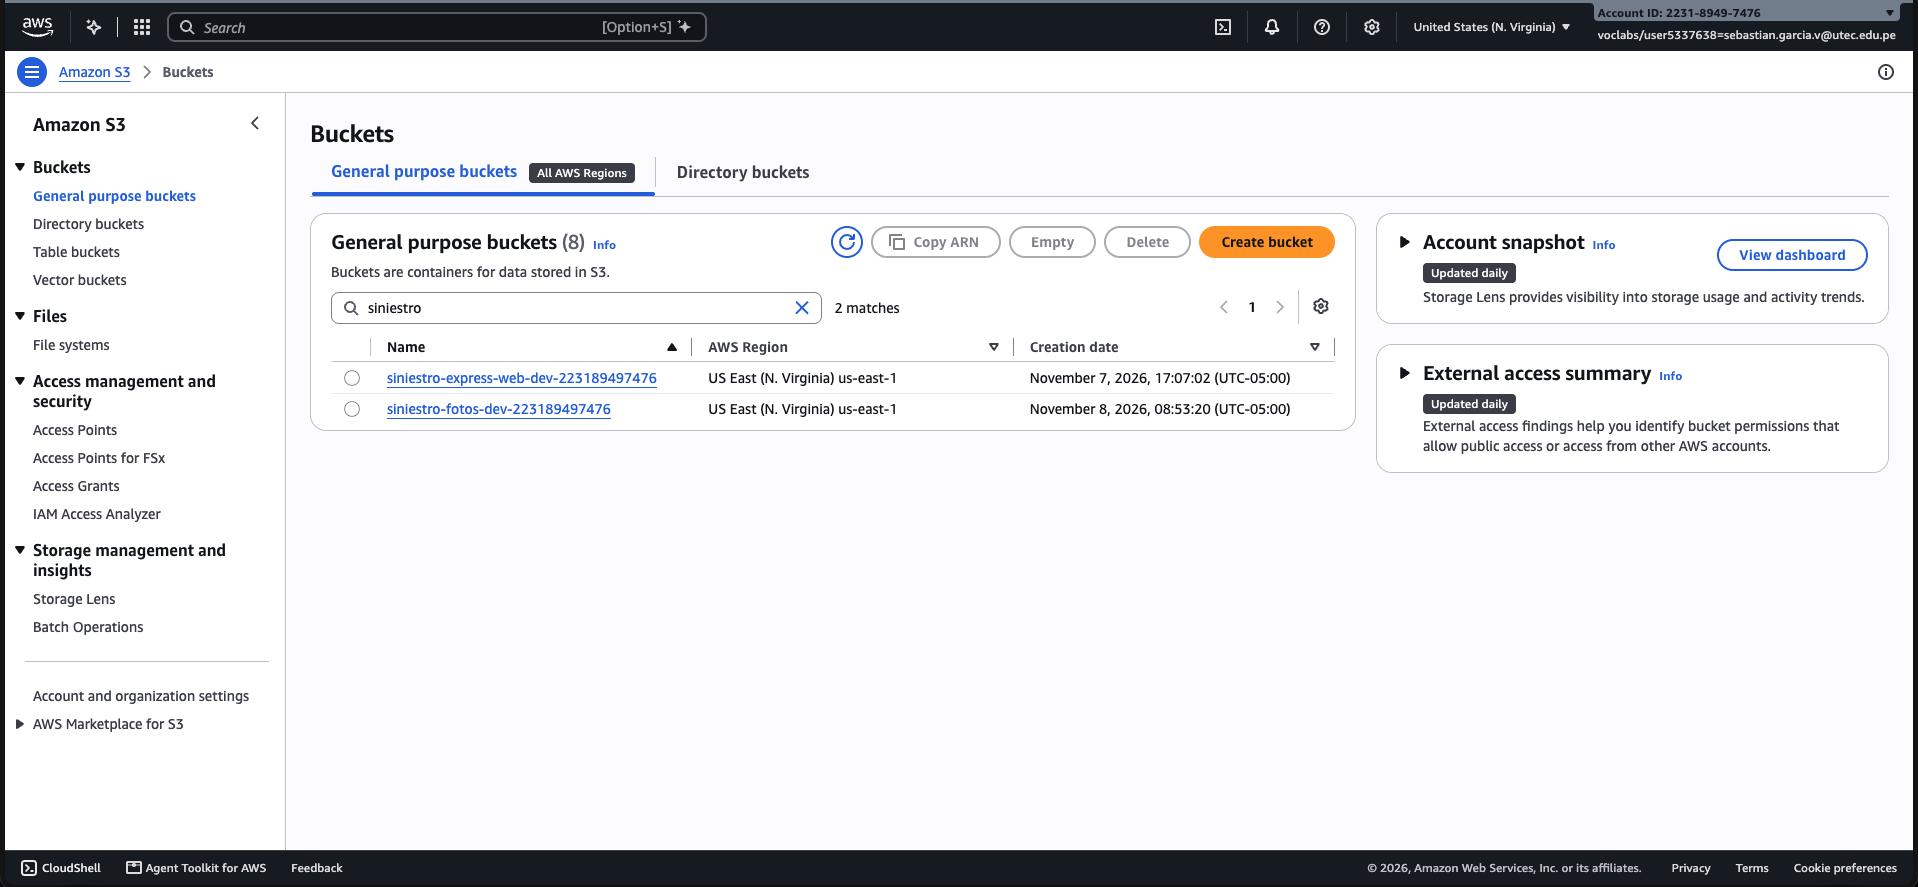
\includegraphics[width=0.95\textwidth]{img/aws_s3.png}
\caption{Los dos buckets: sitio web y fotos}
\label{fig:s3}
\end{figure}

\subsection{Frontend conectado}

El sitio publicado consume las APIs reales. No existe un modo de demostración: si las
variables de entorno faltan, la aplicación muestra un aviso en pantalla en lugar de
inventar respuestas. Las capturas de las figuras \ref{fig:inicio} a \ref{fig:movil}
provienen de ese despliegue.

\begin{figure}[htbp]
\centering
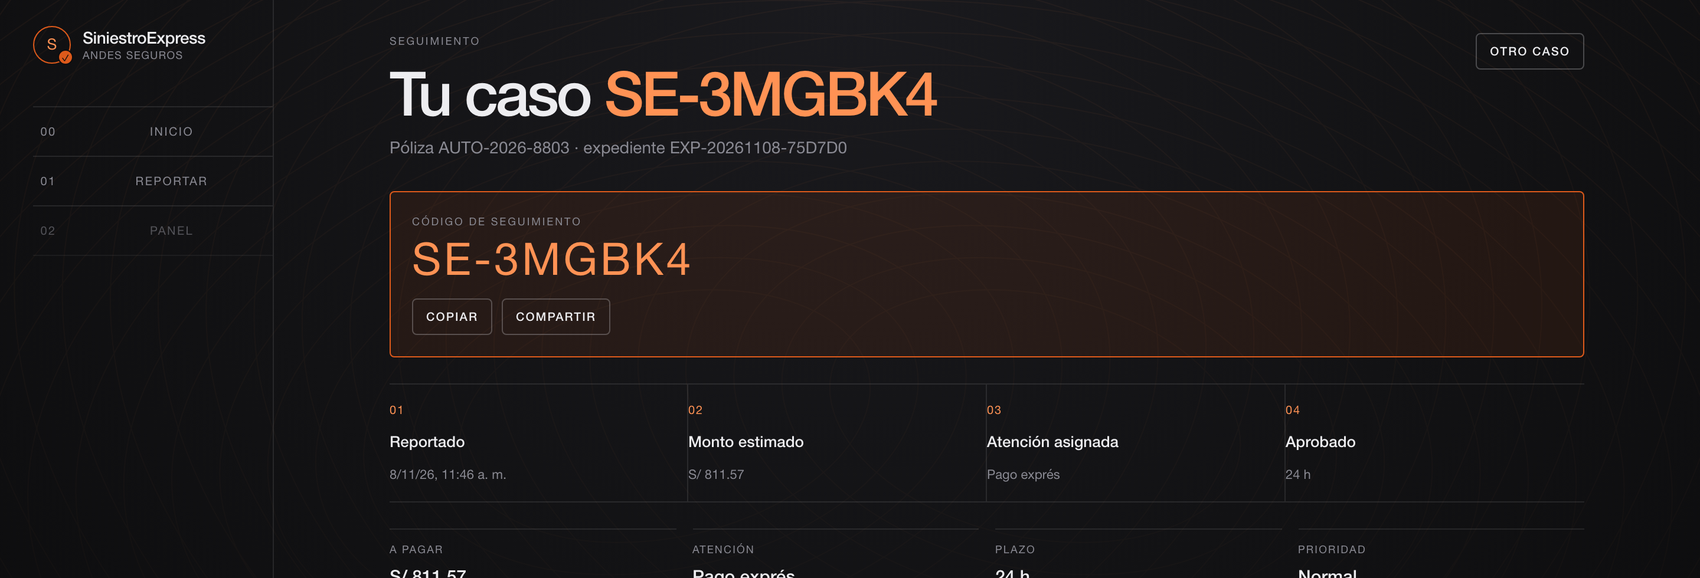
\includegraphics[width=0.92\textwidth]{img/app_seguimiento.png}
\caption{Seguimiento del caso con fotos y conversación}
\label{fig:caso}
\end{figure}

\subsection{Pruebas}

\begin{table}[H]
\centering
\caption{Pruebas automatizadas}
\label{tab:pruebas}
\small
\begin{tabular}{p{4.0cm}p{1.8cm}p{7.4cm}}
\toprule
\textbf{Suite} & \textbf{Casos} & \textbf{Qué cubre} \\
\midrule
\code{services/ml} & 4 & Inferencia, validación de campos y límites de piezas \\
\code{services/core} & 25 & Reglas de decisión, deducible, pérdida total y máquina de estados \\
\code{services/agente} & 15 & Normalización de slots, alias y detección del parte policial \\
\code{tests} & 6 & Integración con DynamoDB simulado y flujo completo \\
\midrule
\textbf{Total} & \textbf{50} & \\
\bottomrule
\end{tabular}
\end{table}

\subsection{Repositorios}

\begin{sloppypar}
\begin{itemize}[itemsep=4pt, leftmargin=*]
  \item \textbf{Código.} \code{github.com/UTEC-AII/siniestro-express} (público).
  \item \textbf{Sitio publicado.}\\ \url{http://siniestro-express-web-dev-223189497476.s3-website-us-east-1.amazonaws.com}
  \item \textbf{Colección de Postman.} \code{docs/postman}, dentro del mismo repositorio.
\end{itemize}
\end{sloppypar}

\clearpage
\section{Conclusiones}

El proyecto demuestra que un trámite de seguros puede resolverse en una conversación sin
perder el control de la decisión. Esa fue la apuesta de diseño y se sostuvo de punta a
punta: el modelo de lenguaje entiende el relato y redacta, pero el monto, la ruta y el
plazo salen de un módulo de reglas que se lee en una pantalla, se prueba con 25 casos y se
puede auditar. Un ajustador puede discutir por qué un siniestro se pagó en 24 horas y otro
fue a peritaje sin abrir el código del agente.

El segundo aprendizaje es de ingeniería. Servir un modelo de machine learning en Lambda no
obliga a llevar la biblioteca de entrenamiento. Exportar los bosques a JSON y recorrerlos
con la biblioteca estándar bajó el paquete de 71 MB a 2,4 MB, mantuvo la latencia en 0,2 ms
y no perdió precisión, con una diferencia máxima de medio céntimo sobre 500 casos. La
condición para que eso funcione es respetar la precisión numérica del entrenamiento:
scikit-learn recorre los árboles en \code{float32}, y un runtime en doble precisión cambia
el monto.

El tercer aprendizaje es de producto, y no estaba en ningún requisito. El agente cerraba
bien la conversación pero mostraba el costo de reparación como si fuera el monto a cobrar;
el asegurado veía una cifra y el analista otra. Corregirlo fue una línea de código y el
cambio más grande en claridad de todo el sistema. Lo mismo pasó con la salida del chat: sin
un botón hacia el seguimiento, el asegurado quedaba en una conversación cerrada sin saber
qué hacer.

En dinero, el resultado es fácil de resumir: la infraestructura cuesta 2.38 USD al mes para
1,900 casos, unos 0.00125 USD por caso, y absorbe alrededor de 1.2 horas de trabajo
administrativo por siniestro. La cuenta no cierra si se presenta como un reemplazo del
analista, porque no lo es; cierra cuando se lee como lo que es, un cambio en dónde se
invierte el tiempo de las personas.

Lo que el proyecto no resuelve también hay que decirlo. Los modelos se entrenaron con datos
sintéticos, así que los montos son coherentes entre sí pero no son precios de mercado. El
panel usa un código de demostración en lugar de autenticación real. Y las fotos sirven como
evidencia, no como fuente de estimación. Son tres límites conocidos, no tres sorpresas.

\subsection*{Trabajo futuro}

\begin{itemize}[itemsep=1pt, topsep=2pt, leftmargin=*]
  \item Reentrenar con el historial real y recalibrar los umbrales.
  \item Autenticación con Cognito y roles para el analista.
  \item Detección de daño desde la foto, hoy solo evidencia.
  \item Asignación de taller por disponibilidad y zona.
\end{itemize}

\end{document}
